\documentclass[UTF8]{ctexart}
\usepackage{xcolor}
\usepackage{enumerate}
\usepackage{graphicx}
\usepackage{geometry}
\usepackage{graphicx} %插入图片的宏包
\usepackage{float} %设置图片浮动位置的宏包
\usepackage{subfigure} 
\usepackage[colorlinks,linkcolor=blue]{hyperref}
\usepackage{mathtools}
\usepackage{listings}
\lstset{ %
    language=python,                % the language of the code
    basicstyle=\footnotesize,           % the size of the fonts that are used for the code
    numbers=left,                   % where to put the line-numbers
    numberstyle=\tiny\color{gray},  % the style that is used for the line-numbers
    stepnumber=2,                   % the step between two line-numbers. If it's 1, each line 
                                    % will be numbered
    numbersep=5pt,                  % how far the line-numbers are from the code
    backgroundcolor=\color{white},      % choose the background color. You must add \usepackage{color}
    showspaces=false,               % show spaces adding particular underscores
    showstringspaces=false,         % underline spaces within strings
    showtabs=false,                 % show tabs within strings adding particular underscores
    frame=single,                   % adds a frame around the code
    rulecolor=\color{black},        % if not set, the frame-color may be changed on line-breaks within not-black text (e.g. commens (green here))
    tabsize=2,                      % sets default tabsize to 2 spaces
    captionpos=b,                   % sets the caption-position to bottom
    breaklines=true,                % sets automatic line breaking
    breakatwhitespace=false,        % sets if automatic breaks should only happen at whitespace
    title=\lstname,                 % show the filename of files included with \lstinputlisting;
                                    % also try caption instead of title
    keywordstyle=\color{blue},          % keyword style
    commentstyle=\color{green},       % comment style
    stringstyle=\color{red},         % string literal style
    escapeinside={\%*}{*)},            % if you want to add LaTeX within your code
    morekeywords={*,...}               % if you want to add more keywords to the set
}
\geometry{left = 2.5cm,right= 2cm}
\title{Chapter 2 \\End to End Machine Learning}
\author{DuLi}
\date{\today}
\begin{document}
\maketitle
\newpage
\tableofcontents
\newpage
\section{Outline}
\setlength{\parskip}{0.5em} 

Here are main steps you will go through:
\begin{itemize}
	\item[1.] Look at the big picture.
	\item[2.] Get the data.
	\item[3.] Discover and visualize the data to gain insights.
	\item[4.] Prepare the data fpr machine learning algorithms.
	\item[5.] Select a model and train it.
	\item[6.] Fine-tune your model.
	\item[7.] Present your solution.
	\item[8.] Launch,monitor,and maintain your system.
\end{itemize}
\section{Working with Real Data}
Here are a afew places you can look to get data:
\begin{itemize}
	\item Popular open data open repositories:
		\item[-] UC Irvine Machine Learning Repositories.
		\item[-] Kaggle datasets.
		\item[-] Amazon's AWS datasets.
	\item Meta Portals(they list open data repositories)
		\item[-] dataportals.org
		\item[-] opendatamonitor.eu
		\item[-] quandl.com
	\item Other pages listing many popular open data repositories
		\item[-] Wikipedia's list of Machine Learning datasets.
		\item[-] Quora.com question.
		\item[-] Datasets subreddit.
\end{itemize}

\begin{figure}[H]
\centering
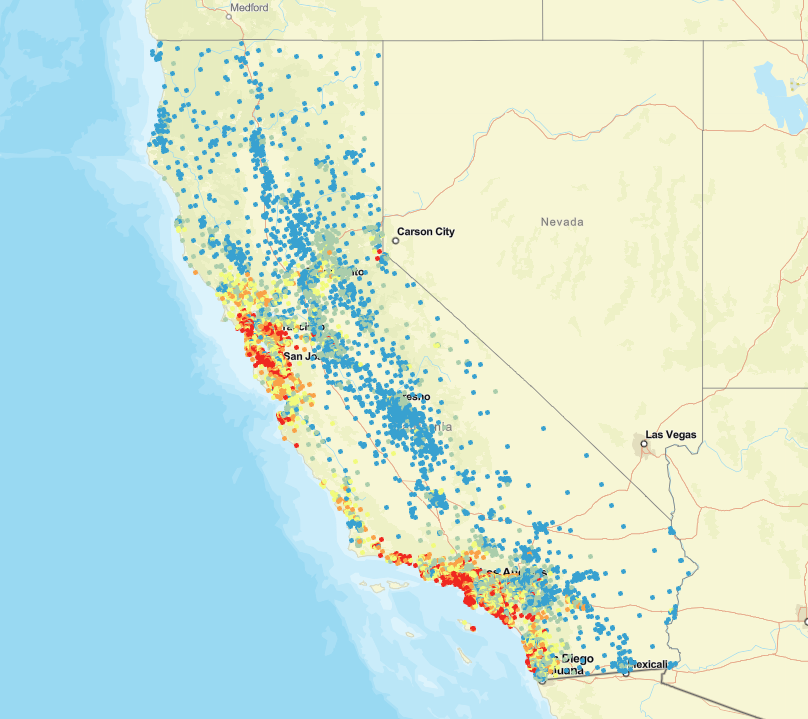
\includegraphics[width = 4in]{picture.png}
\caption{California Housing Prices Databases}
\end{figure}

\section{Look at the Big Picture}
\subsection{Frame the Problem}
The first question to ask you is what exactly is the bussiness objective;building a model is probably not the end goal.How do you expect use and benefit from this model?This is improtant because it will determine how you frame the problem,what algorithms you will select,what performance measure you will use to evaluate your model,and how much effort you should spend tweaking it.
Your model output (a predicting of a district's median housing price) will be fed to another Machine Learning system along with many other signals.This downstream system will determine whether it is worth investing in a given area or not.

\begin{figure}[H]
\centering
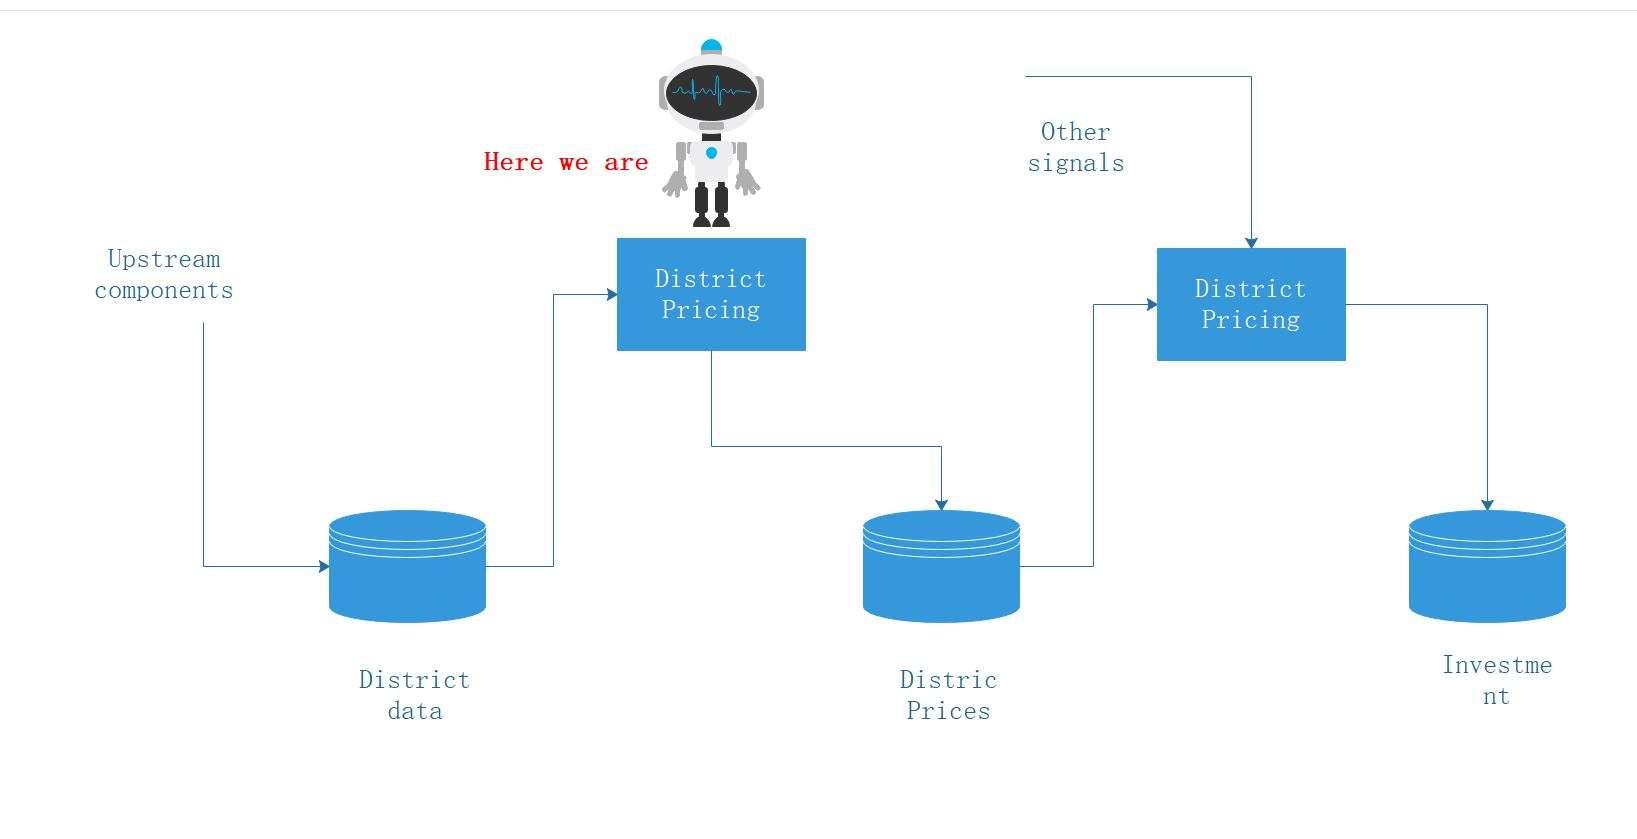
\includegraphics[width = 4in]{PROCESS.JPG}
\caption{A machine learning pipeline for real estate investment}
\end{figure}

The next step is framing the problem:is it supervised,unsupervised,or Reinforcement learning?Is it a classification task,a regression task,or something else?Should we use batch learning or online learning technique?
Clearly it is supervised,we need historical data to train the model.Moreover it is a typical regression task,more specifically,this is a multivariate regression since the system will use mutiple features to make a prediction.In first chapter,we predicted life satisfiction based on just one feature,the GDP per captia.Finally,there is no continuous flow of data coming in the system,there is no particular need to adjust to changing data rapidly,and the data is small enough to fit in memory,so plain batch learning should do just fine.

\subsection{Select a Performance Measure}
The next step is to select a performance measure.A typical performance measure for regression problems is the Root Mean Square Error(均方根误差),it measures the standard deviation of the errors the system makes in its prediction.

\begin{equation}
RMSE(X,h) = \sqrt{\frac{1}{m}\sum_{i=1}^{m}(h(X^{i})-y^{i})^{2}}
\end{equation}

Even though the RMSE is generally the perferred performance measure for regression tasks,in some contexts you may prefer to use another function.For example,suppose that there are many outlier districts.In that case,we may consider using the Mean Absolute Error(平均绝对误差):
\begin{equation}
	MAE(X,h) = \frac{1}{m}\sum_{i=1}^{m}|h(X^i)-y^i|
\end{equation}

Both the RMSE and MAE are ways to measure the \emph{distance} between two vectors.Various distance measures or norms are possible:
\begin{itemize}
	\item Euclidean norm(欧几里得距离)。
	\item Manhattan norm(曼哈顿距离),it measures the distance between two points in a city if you can only travel along orthogonal city blocks.也就是指城市中两点之间沿着街区边缘走路的距离。
	\item More generally,the $l_{k}$ norm of a vector $v$ containing n elements is defined as:
	\begin{equation}
		\parallel v \parallel = (\mid v_{o} \mid^k + \mid v_{1} \mid^k+ \cdots + \mid v_{n} \mid^k)^\frac{1}{k} 
	\end{equation}
\end{itemize}

\section{Get the data}
It's time to get your hands dirty.
\subsection{Create the workspace}
First,you need to have Python enviornment installed.We recommand you installed anaconda on your computer.\url{https://www.anaconda.com/}
\subsection{Take a Quick Look at the Data Structure}
Let's take a look a the Data Structure.I download the database from Kaggle.\url{https://www.kaggle.com/camnugent/california-housing-prices}.Let's take a glance of the data structure.
Each row represent one district.There are 10 attributes(Figure 3):longitude,lattidute,housing\underline{ }median\underline{ }age,total\underline{ }\\rooms,total\underline{ }bedrooms,population,households,median\underline{ }income,median\underline{ }house\underline{ }value,ocean\underline{ }proximity.

\begin{figure}[H]
\centering
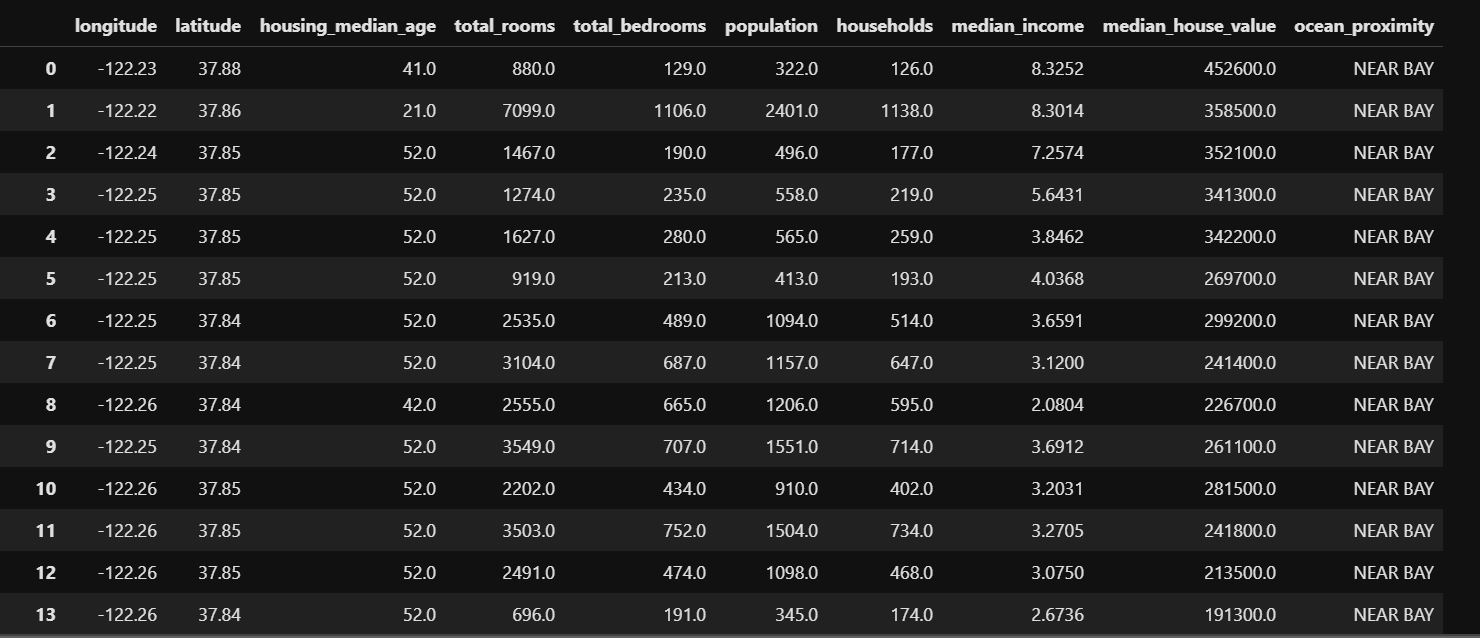
\includegraphics[width = 4in]{DataStructure.JPG}
\caption{Data Structure}
\end{figure}

The info method is useful to get a quick description of the data,in particular the total number of rows,and each attribute's type and number of non-null values.There are 20640 instances in the dataset,which means that it is fairly small by Machine Learning standards,but it's perfect to get started.Notice that the total\underline{ }bedrooms attribute has only 20433 non-null values,meaning that 207 districts are missing this feature.We will need to take care of this later.

\begin{figure}[H]
\centering
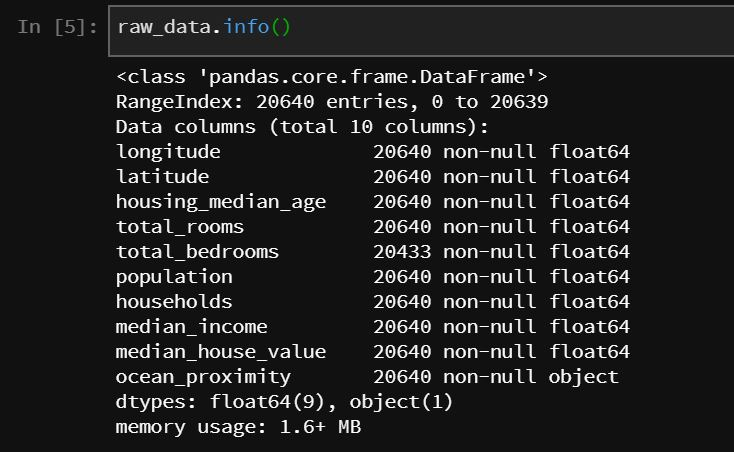
\includegraphics[width = 4in]{datainfo.JPG}
\caption{Data Info}
\end{figure}

All attribute are numercial,except the ocean\underline{ }proximity field.We can find out what categories exist and how many districts belong to each category by using the value\underline{ }counts() method:

\begin{figure}[H]
\centering
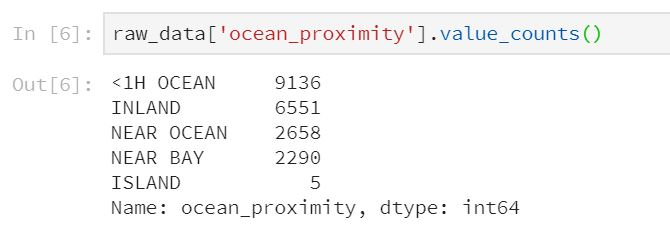
\includegraphics[width = 3in]{datacounts.JPG}
\caption{Data Counts}
\end{figure}

Let's look at the other fields.The describe() method shows a summary of the numercial attributes.(Figure 6).The count,mean,min and max rows are self-explanatory.

\begin{figure}[H]
\centering
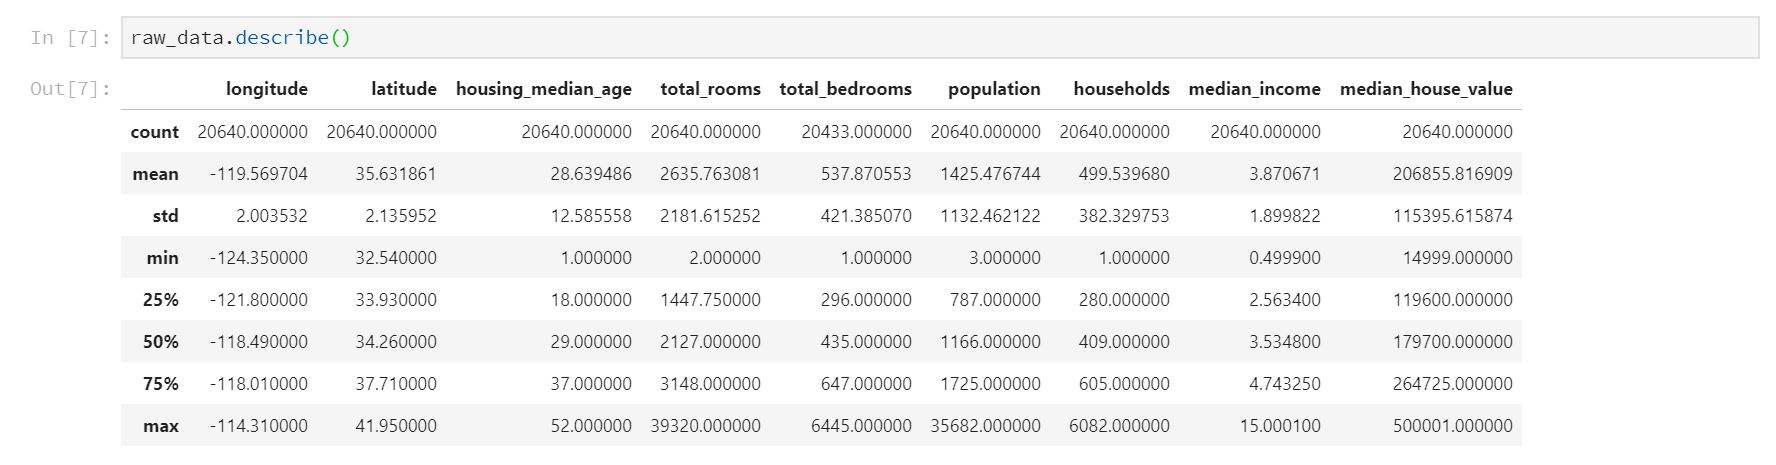
\includegraphics[width = 4in]{DATADESCRIBE.JPG}
\caption{Data Describe}
\end{figure}

Another quick way to get a feel of the type of data you are dealing with is to plot a histogram for each numercial attribute.

\begin{figure}[H]
\centering
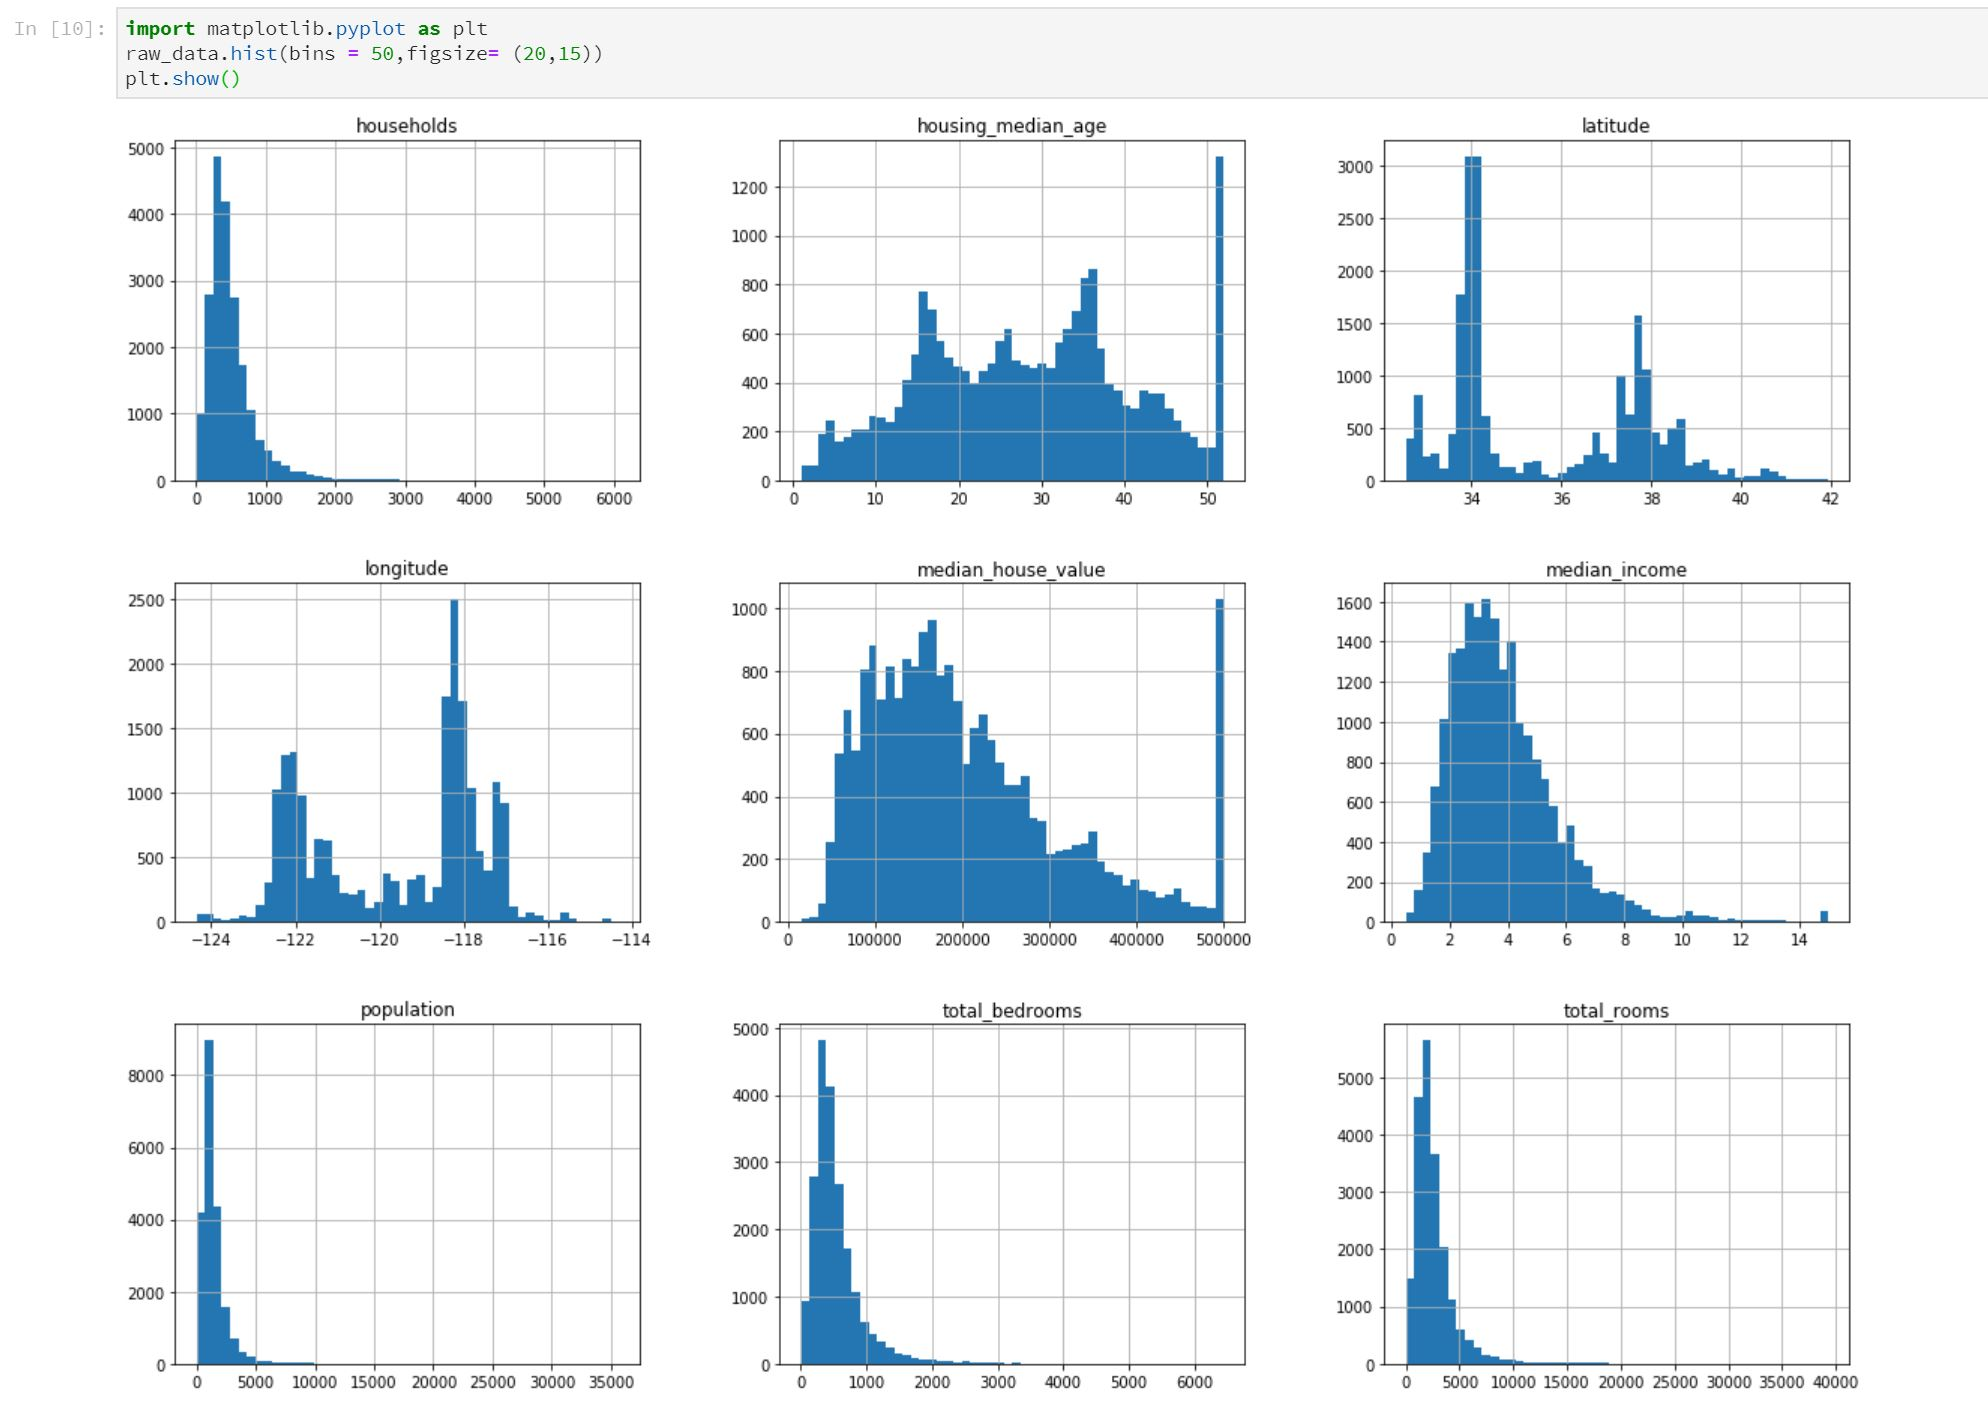
\includegraphics[width = 3.5in]{datahist.JPG}
\caption{A histogram for each numercial attribute}
\end{figure}

\subsection{Create a Testset}

Create a test set is theoretically quite simple:just pick some instances randomly,typically 20\% of the dataset,and set them aside.

\begin{lstlisting}
import numpy as np

def split_train_test(data,test_ratio):
	shuffled_indices = np.random.permutation(len(data))
	test_set_size = int(len(data)*test_ratio)
	test_indices = shuffled_indices[:test_size]
	train_indices = shuffled_indices[test_size:]
	return data.iloc[train_indices],data.iloc[test_indices]

\end{lstlisting}

We can then using the function like this:
\begin{lstlisting}
train_set,test_set = split_train_test(housing,0.2)
\end{lstlisting}

This works,but it not perfect:if you run the program again,it will generate a different test set.One solution is to save the test set on the first run and then load it in subsequent runs.Another option is to set the random number generate's seed(eg. np.random.seed(52))before calling np.permutation().But both these solution will break next time you fetch an updated dataset.A common solution is to use each instance's identifier to decide whether or not it should go in the test set.For example,you could compute a hash of each instance's identifier.

\begin{lstlisting}
import hashlib

def test_set_check(identifier,test_ratio,hash):
    return hash(np.int64(identifier).digest()[-1]<256*test_ratio)

def split_train_test_by_id(data,test_ratio,id_column,hash=hashlib.md5):
    ids = data[id_column]
    in_test_set = ids.apply(lambda id_:test_set_check(id_,test_ratio,hash))
    return data.iloc[~in_test_set],data.iloc[in_test_set]
\end{lstlisting}

Unfortunately,the hosuing dataset does not have an identifier column.The simplest solution is to use the row index as the ID:
\begin{lstlisting}

housing_with_id = housing.reset_index()
train_set,test_set = split_train_test_by_id(hosuing_with_id,0.2,"index")

\end{lstlisting}


We can utilize the train\underline{ }test\underline{}split function to reah the same effect of the split function above.

\begin{lstlisting}
from sklearn.model_selection import train_test_split

train_set,test_set = train_test_split(housing,test_size = 0.25,random_state = 0)

\end{lstlisting}
This generally fine if your dataset is large enough,bu if it is not,you run the risk of introducing a significant sampling bias.For example,when a survey company decides to call 1000 people to ask them a few questions ,they don't just pick 1000 people randomly in a phone booth.They try to ensure that these 1000 people are representative of the whole population,eg. the US population is composed of 51.3\% female and 48.7\% male,so a survey in the US should try to maintain this ratio in the sample:513 female and 487 male.This is called \emph{stratified sampling.}

Since the median income is a very important attribute to predict median housing prices. You may want to ensure that the test set is representative of the various categories of incomes in the whole dataset 

\begin{figure}[H]
\centering
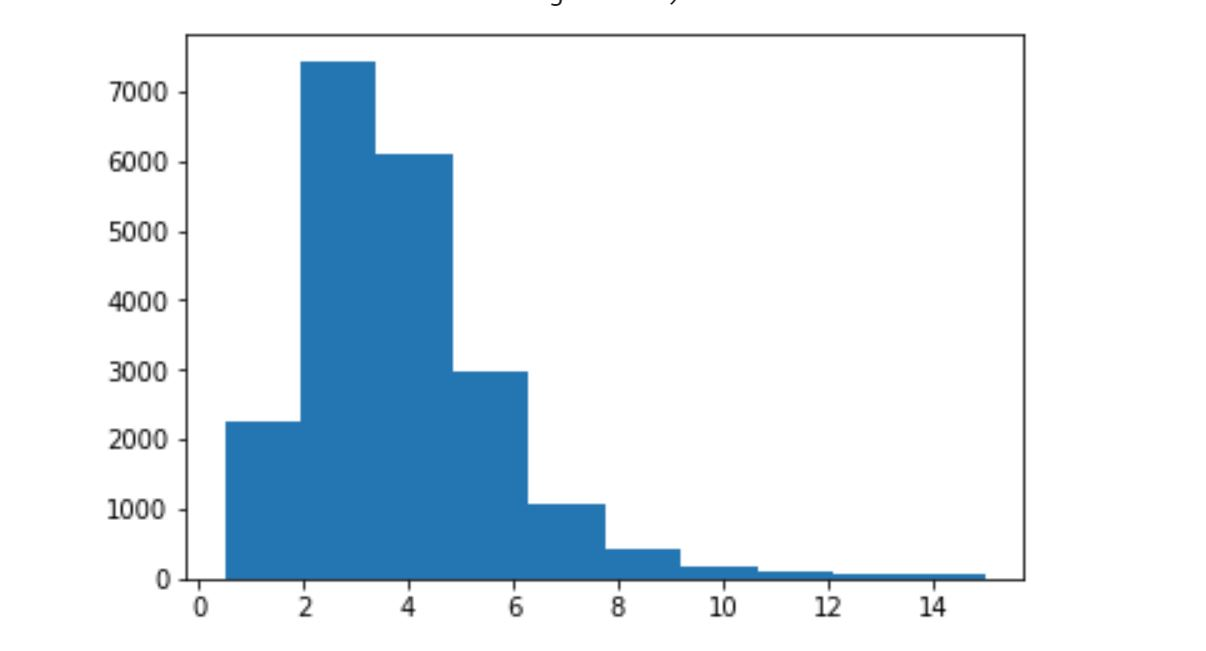
\includegraphics[width = 4in]{incomehist.JPG}
\caption{Histogram of income categories}
\end{figure}

Let's look at the histogram of income categories,most median income values are clustered around 2-5(tens of thousands of dallors),but some median incomes go far beyond 6.It is important to have a sufficient number of instances in your dataset for each stratum,or else the estimate of the stratum'simportance may br biased,so we should not have too many strata(dividing the median income by 1.5 and rounding up using cel and then merge all the categories greater than 5 into category 5).

\begin{lstlisting}
raw_data["income_cat"] = np.ceil(raw_data["median_income"]/1.5)
raw_data["income_cat"].where(raw_data["income_cat"]>5,5.0,inplace = False)
\end{lstlisting}

Now you are ready to do stratified sampling based on the income category.For this we can use Scikit-learn's StratifiedShuffleSplit class:

\begin{lstlisting}
from sklearn.model_selection import StratifiedShuffleSplit

split = StratifiedShuffleSplit(n_splits = 1,test_size = 0.2, random_state = 17)

for train_index, test_index in split.split(raw_data, raw_data["income_cat"]):
    strat_train_set = raw_data.loc[train_index]
    strat_test_set = raw_data.loc[test_index]	
\end{lstlisting}

By this way,the category proportions in the test\underline{ }set which generated with stratified sampling almost identical to those in the full dataset.

We spent quite a bit of time on the test set generation for a good reason:this is an often neglected but critical part of a Machine Learning project.
At last,we should remove the income\underline{ }cat attribute so the data is back to its original state:

\begin{lstlisting}
for set in(strat_train_set,strat_test_set):
	set.drop(["income_cat"],axis = 1,inplace = True)
\end{lstlisting}


这个部分看似平淡无奇,其实还蛮有用的,之前在选数据集的时候,从来没有考虑过这个问题。回头想想,选择有代表性的数据集对于一个监督学习的系统来说,还是非常重要的。使得在训练阶段也能提高精度,这个道理我想是不言自明的。

\section{Discover and Visualize the Data to Gain Insights}

So far we have only taken a quick glance at the data to get a general understanding of the kind of data we are manipulating.In our case,the set is quite small so you can just work directly on the full set.Let's create a copy so you can play with it without harming the training set.

\begin{lstlisting}
housing = strat_train_set.copy()
\end{lstlisting}

\subsection{Visualizing Geographical Data}

Since there is geographical information(latitude and longitude),let's plot it!

\begin{lstlisting}
housing.plot(kind="scatter",x="longitude",y="latitude")
\end{lstlisting}

\begin{figure}[H]
\centering
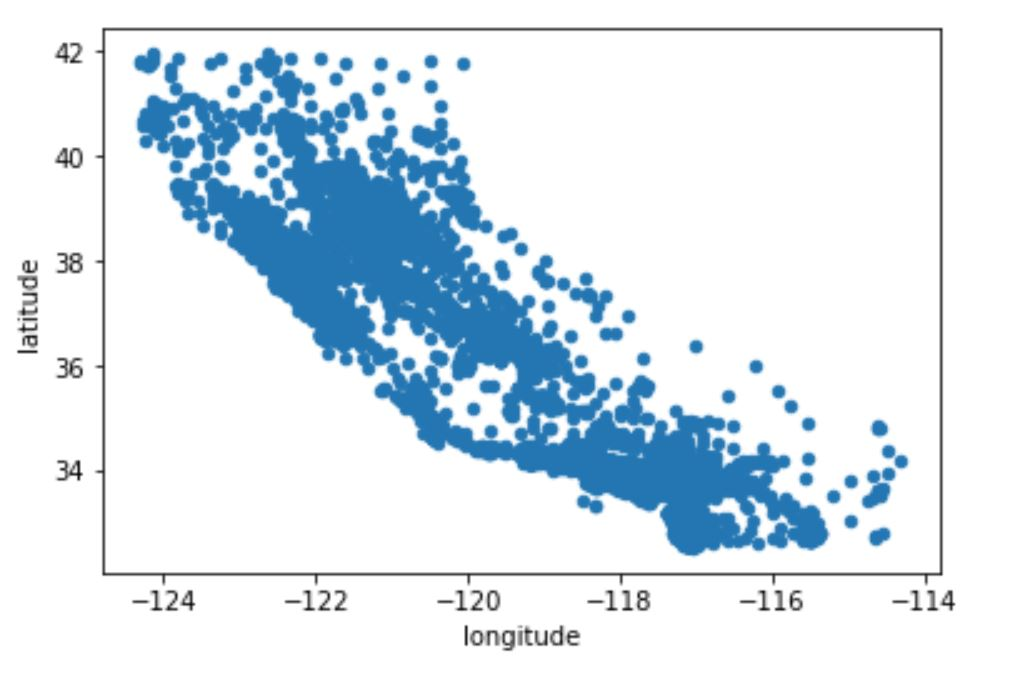
\includegraphics[width = 4in]{longi_and_lati.JPG}
\caption{A geographical scatterplot of the data}
\end{figure}

Setting the alpha option to 0.1 makes it much easier to visualize the places where there is a high density of data points.

\begin{lstlisting}
housing.plot(kind="scatter",x="longitude",y="latitude",alpha = 0.1)
\end{lstlisting}

alpha:float (0.0 transparent through 1.0 opaque),这里的alpha指的是透明度,所以密度越大的地方,因为重叠的原因,颜色就会越深。

It's better now,let's look at the housing prices.The radius of each circle represents the district's population(option s),and the color represents the price(option c).We will use a predefined color map(option cmap)called jet,which ranges from blue(low values) to red(high prices):

\begin{lstlisting}
housing.plot(kind="scatter",x="longitude",y="latitude",alpha=0.4,s=housing["population"]/100,label="population",c="median_house_value",cmap=plt.get_cmap("jet"),colorbar=True)
plt.legend()
\end{lstlisting}

\begin{figure}[H]
\centering
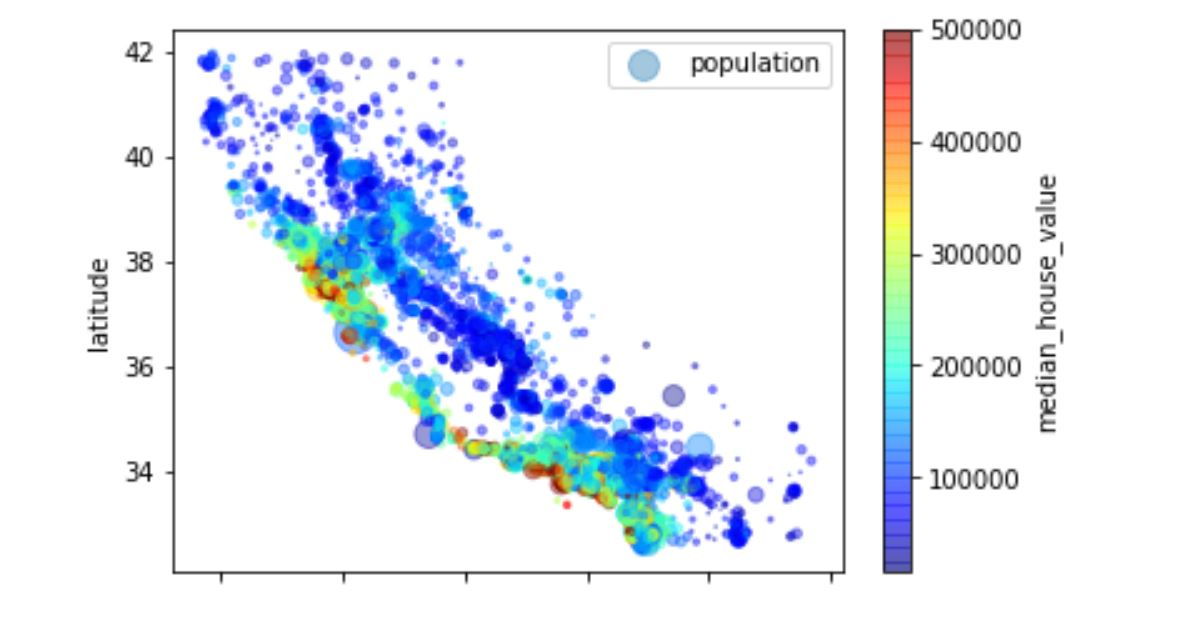
\includegraphics[width = 4in]{Housing_price_pic.JPG}
\caption{California housing prices}
\end{figure}

观察最后得到的图我们大概能看得出一些结论,这些结论也与我们的常识相符。首先,房价和位置的关系很大,临海的房价普遍要高一些,还有某些位置的房价普遍要高一些,这些地方应该是加州沿海的一些城市,旧金山,洛杉矶等等。当然这也不是全部,北部沿海的房价也会低一些。

\subsection{Looking for Correlations}

 Since the data set is not too large ,we can easily compute the \emph{Standard correlation coefficient}(also called Pearson's r 皮尔森相关系数) between every pair of attributes using the corr() method:

\begin{lstlisting}
corr_matrix = housing.corr()
\end{lstlisting}

The matrix is big,so let's look at a specific attribute(eg.median house value).
\begin{lstlisting}
corr_matrix["median_house_value"].sort_values(ascending=False)
\end{lstlisting}

The correlation coefficient ranges from 1 to -1.接近1代表正相关,接近-1代表负相关,我们可以看出平均房价和收入是正相关关系,而和经度是负相关的,也就是内陆房价低,沿海高。Finally,coefficients close to zero mean there is no linear correlation.

\begin{figure}[H]
\centering
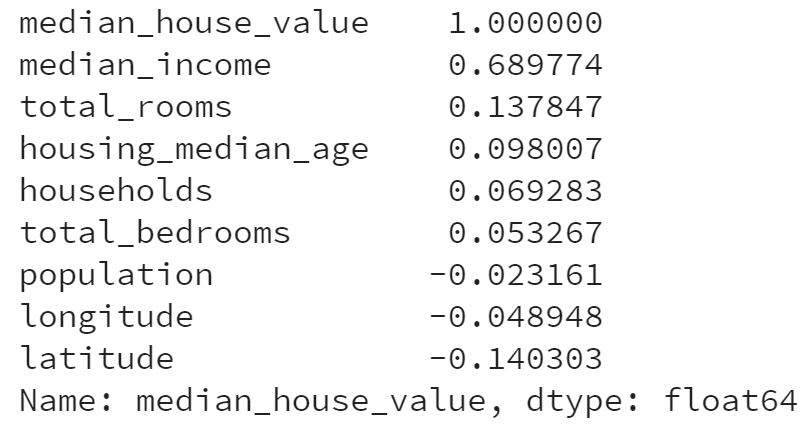
\includegraphics[width = 2.5in]{pearson_r.JPG}
%\caption{California housing prices}
\end{figure}

下面这张图来自维基百科,从左到右依次表示皮尔森相关系数在不同值时的情况。

\begin{figure}[H]
\centering
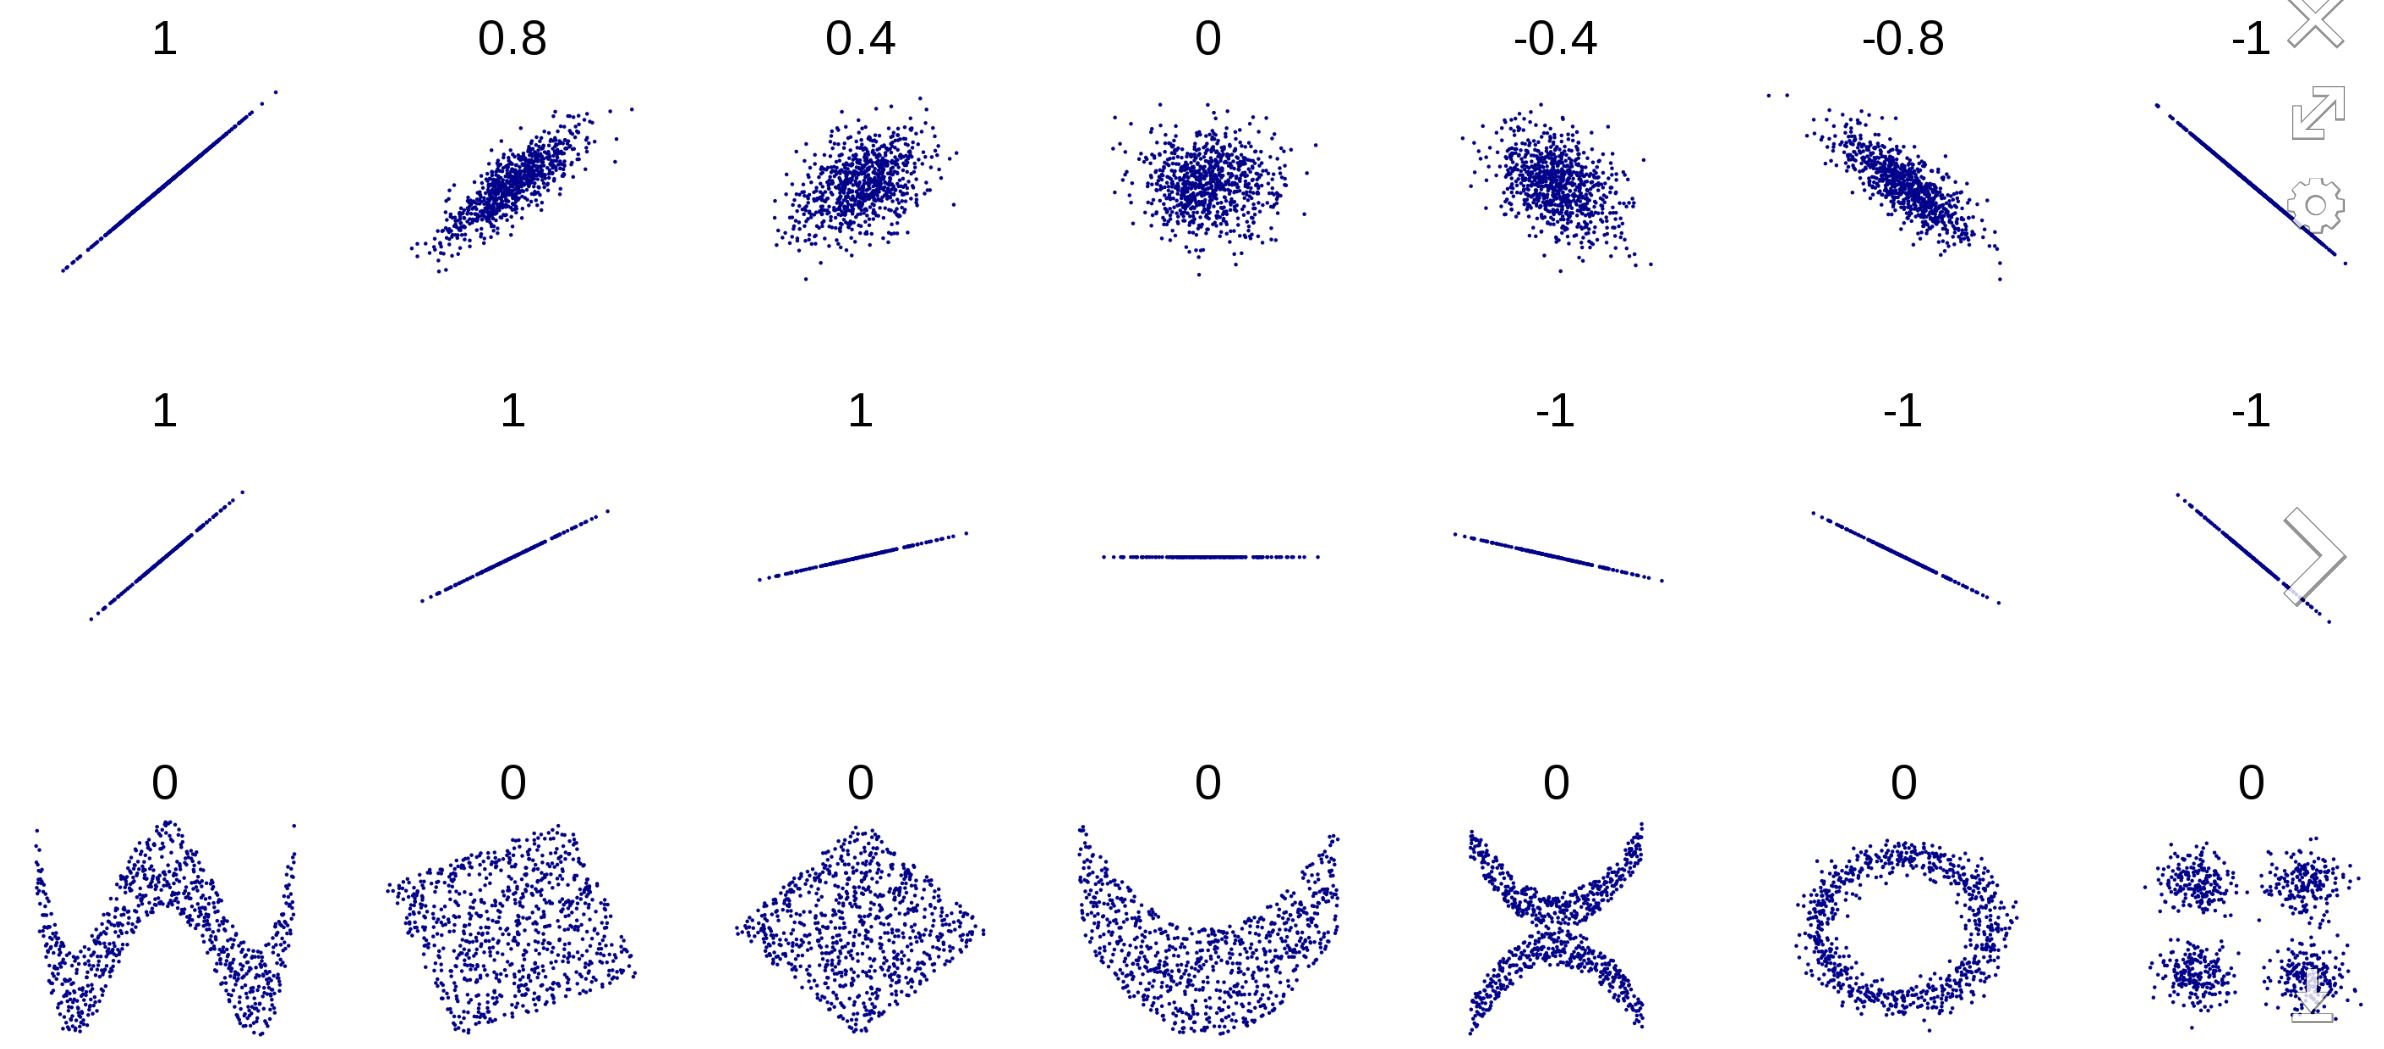
\includegraphics[width = 4in]{scatter_matrix.JPG}
\caption{Scatter Matrix}
\end{figure}

The correlation coefficient only measures linear correlations.

Another way to check for correlations between attributes is to use Pandas' scatter\underline{ }matrix function.Since there are now 11 numerical attributes,you would get $11^2$ plots,so let's just focus on a few promising attributes that seem most correlated with the median housing value.

\begin{lstlisting}
from pandas.plotting import scatter_matrix

attributes = ["median_house_value","median_income","total_rooms","housing_median_age"]

scatter_matrix(housing[attributes],figsize=(12,8))
\end{lstlisting}


\begin{figure}[H]
\centering
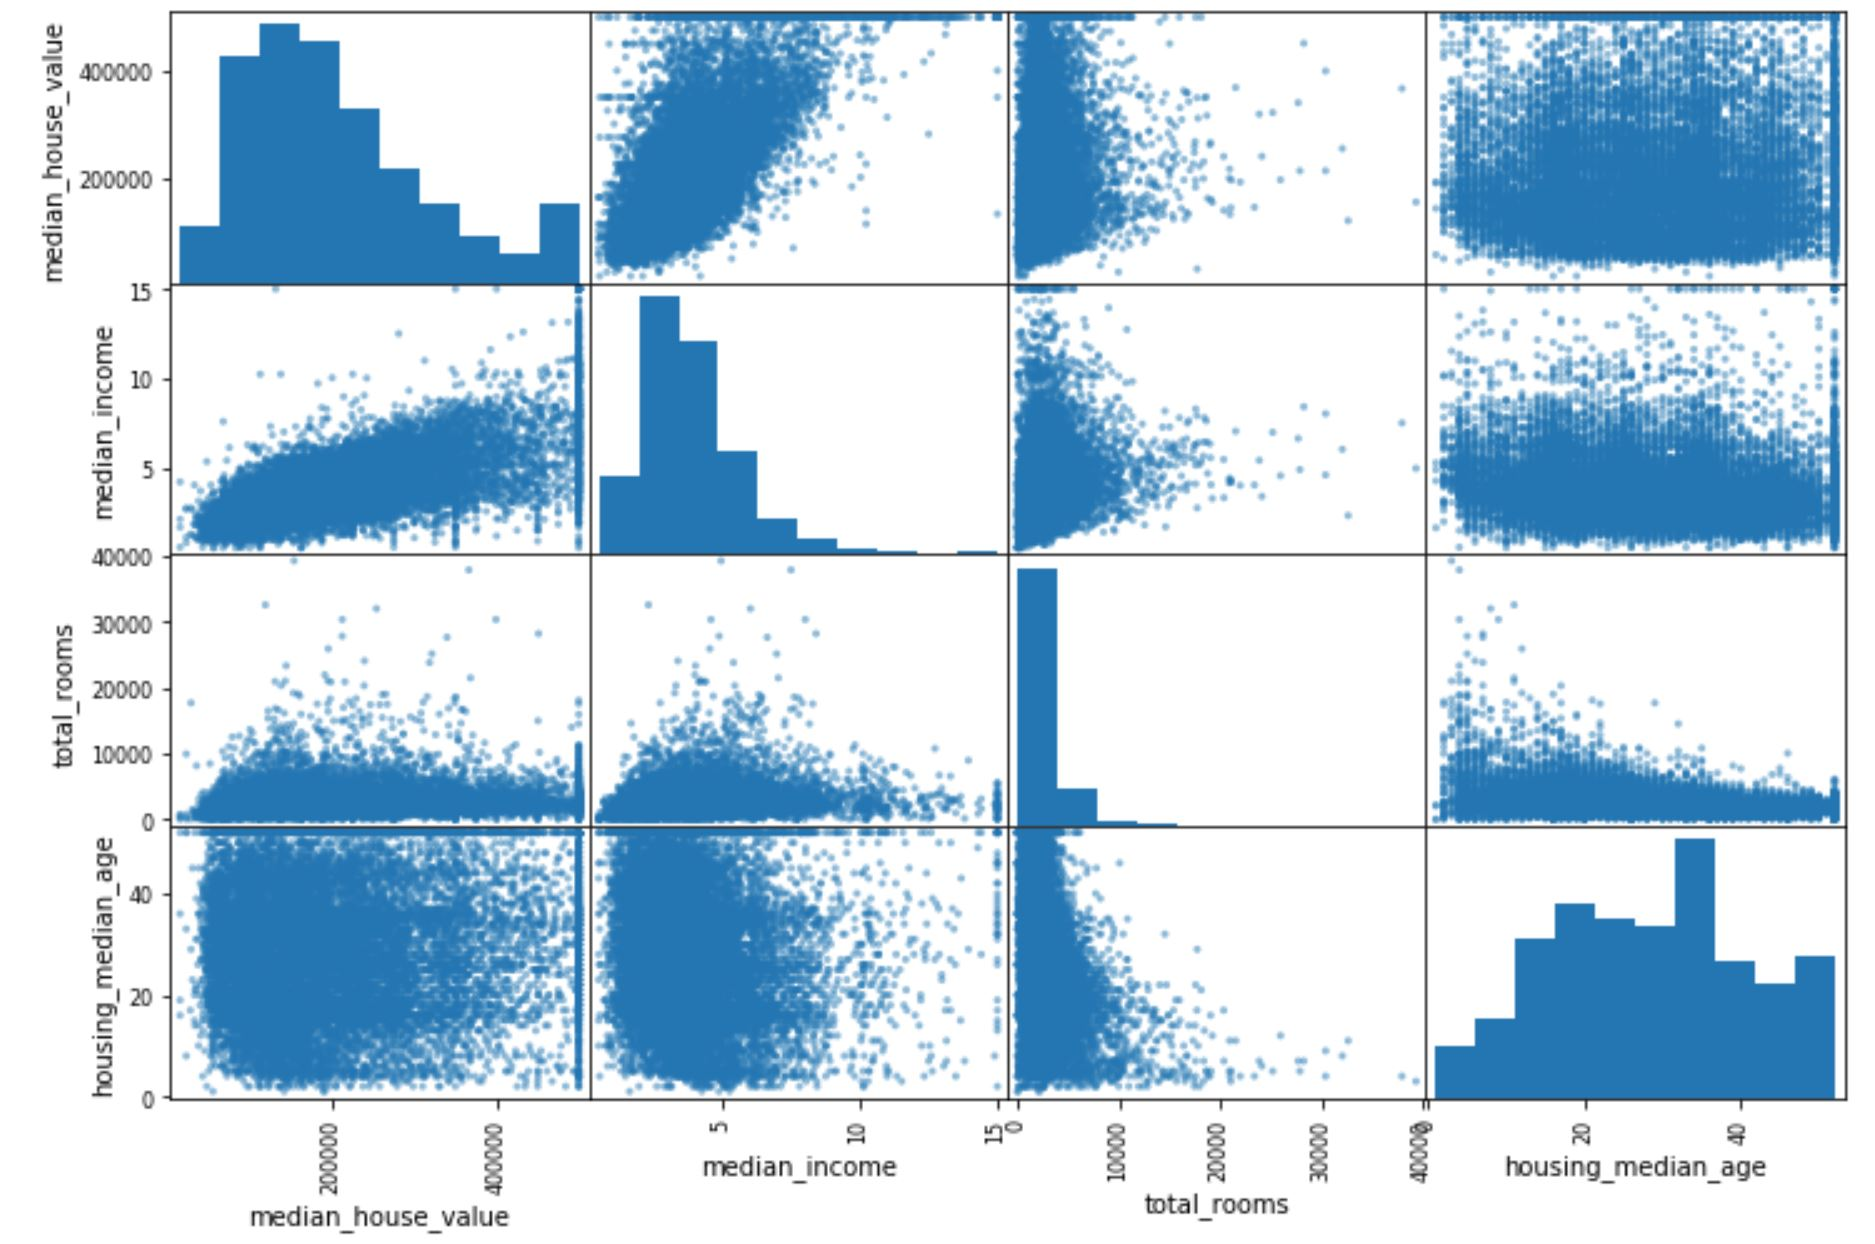
\includegraphics[width = 4in]{scatter_col.JPG}
\caption{Scatter Matrix}
\end{figure}

这里简单做一个说明,之几张图是将数据按照各自的位置两两进行绘图,按照皮尔森系数的意义,两个数据集在一起越接近一条直线,相关性越好,所以在这张图上可以明显的看出,median\underline{ }income参数和median\underline{ }house\underline{ }value的相关性是最好的。这个也和之前计算的结果相符。接下来重点关注这个两个参数之间的关系。
\begin{lstlisting}
housing.plot(kind="scatter",x="median_income",y="median_house_value",alpha = 0.1)
\end{lstlisting}

\begin{figure}[H]
\centering
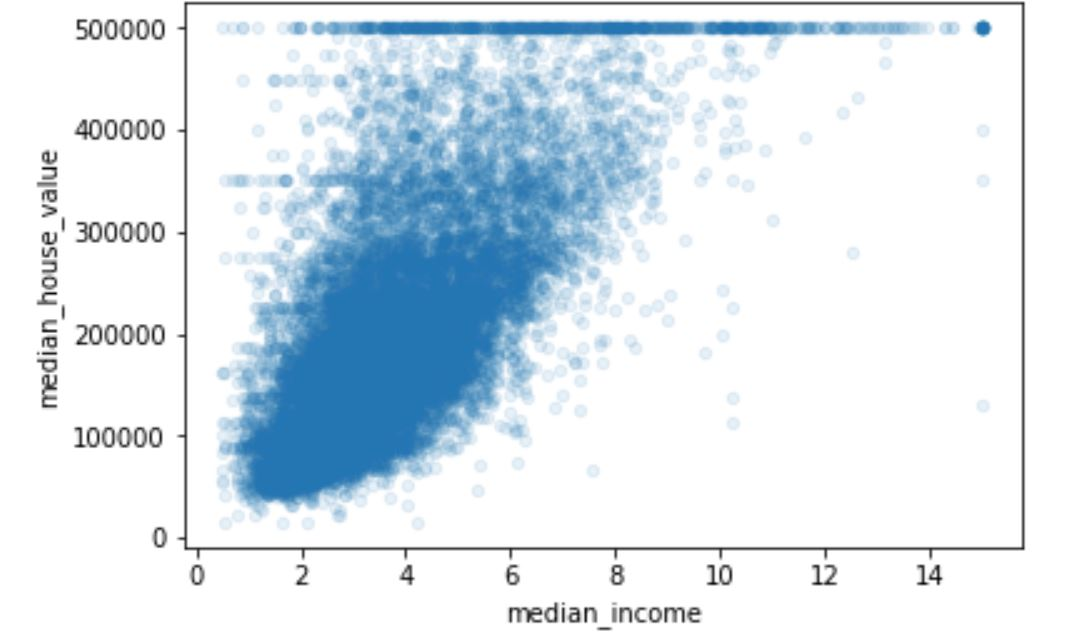
\includegraphics[width = 4in]{specific_scatter.JPG}
\caption{Median income versus median house value}
\end{figure}

This plot reveals a few things.First,the correlation is indeed very strong;we can clearly see the upward trend and the points are not too dispersed.Second,the price cap is clearly visible as a horizontial line at 500000,and this plot reveals other less obvious straight lines:450000,350000.


\subsection{Experinment with attribute Combinations}
One last thingwe may want to do before actually preparing the data for Machine Learning algorithms is try out various attribute combinations.简单的举个例子,就是说单单看一个地区卧室的总数并不是非常有用的,还必须结合房间数或者人口数才真正的有意义。接下来在数据集上,我们把这几个属性添上。

\begin{lstlisting}
housing["roms_per_household"] = housing["total_rooms"]/housing["households"]
housing["bedrooms_per_room"] = housing["total_bedrooms"]/housing["total_rooms"]
housing["population_per_room"] = housing["population"]/housing["total_rooms"]
\end{lstlisting}

接下来再算一次Pearson's r:
\begin{lstlisting}
corr_matrix = housing.corr()
corr_matrix["median_house_value"].sort_values(ascending=False)
\end{lstlisting}

\begin{figure}[H]
  \centering
    \subfigure[Original correlation]{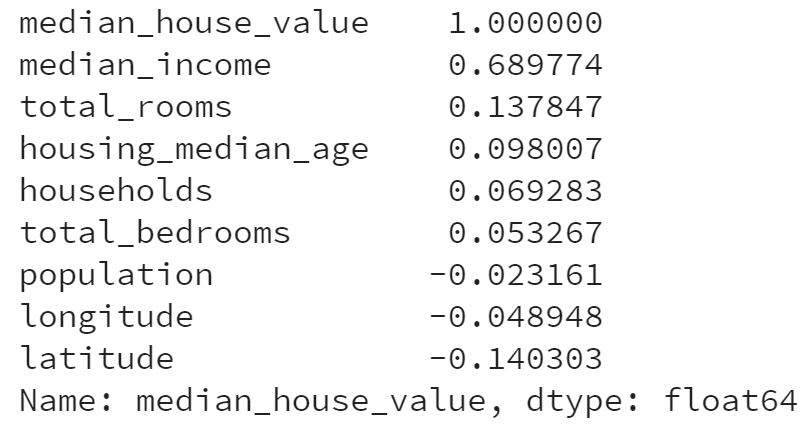
\includegraphics[width=0.5\textwidth]{pearson_r.JPG}}
    \subfigure[Combination correlation]{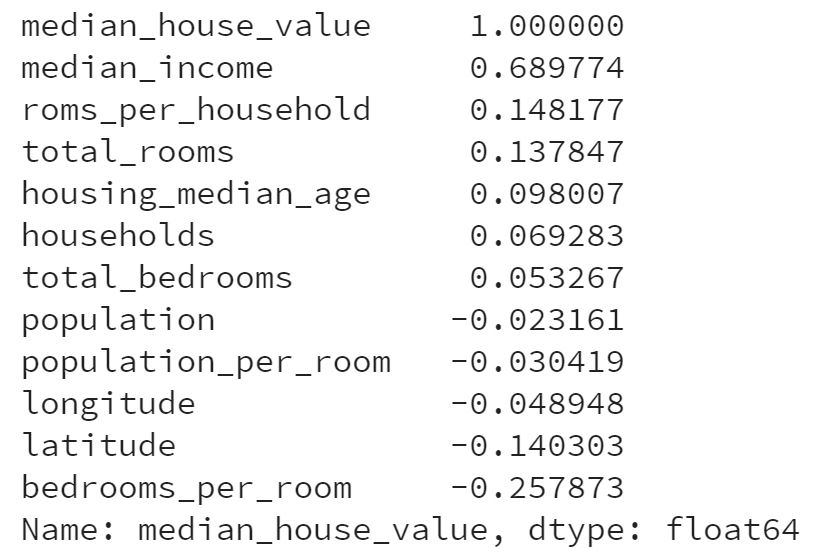
\includegraphics[width=0.44\textwidth]{pearson_R_new.JPG}} \  
    \caption{Comparation of two cases}
    \label{fig:data_distribution}
    \vspace{0.2in}
\end{figure}

值得注意的是,在相关性的计算上,最坏的情况是0,无论是正相关还是负相关都是好的,也就是说越接近1或者-1都好,所以在这里看出,计算后的bedrooms\underline{ }room是好于卧室数以及房间数的。同时,rooms\underline{ }\\household也是同样的情况。在后续我们运行系统之后,会得到比现在更加深入的信息,这是一个迭代并不断优化的过程。

\section{Prepare the Data for Machine Learning Algorithms}

数据预处理是一个重要的过程,是常见的处理过程,在项目和项目之间大概是可以通用的。首先要做的是数剧的分离,即原数据集和label的分离。
\begin{lstlisting}
housing = strat_train_set.drop("median_house_value",axis=1)
housing_labels = strat_train_set["median_house_value"].copy()
\end{lstlisting}
Note that drop() creates a copy of the data and does not affect  strat\underline{ }train\underline{ }set.

\subsection{Data Cleaning}

Most Machine Learning algorithms cannot work with missing features.We noticed that the total\underline{ }bedrooms attribute has some missing values,let's fix this:

\begin{itemize}
	\item Get rid of corresponding districts.
	\item Get rid of the whole attribute.
	\item Set the value to some value(0,mean,median,etc) 
\end{itemize}

We can accomplish these easily using DataFrame's dropna(),drop(),and fillna() methods:

\begin{lstlisting}
housing.dropna(subset=["total_bedrooms"])
housing.drop("total_bedrooms",axis=1)
hosuing["total_bedrooms"].fillna(median)
\end{lstlisting}

Scikit-Learn provide a handy class to take care of missing values:Imputer.Here is how to use it.First,we need to crate an Imputer instance,specifying that you want to replace each attribute's missing values with the median of that attribute:
\begin{lstlisting}
from sklearn.preprocessing import Imputer
imputer = Imputer(strategy="median")
\end{lstlisting}

Since the median can only be computed on numercial attributes,we need to create a copy of the data without the text attribute ocean\underline{ }proximity:

\begin{lstlisting}
housing_num = housing.drop("ocean_proximity",axis = 1)
\end{lstlisting}
Now we can fit the imputer instance to the training data using the fit() method:
\begin{lstlisting}
imputer.fit(housing_num)
\end{lstlisting}
The imputer has simply computed the median of each attribute and stored the result in the statistics\underline{ } instacne varible.
\begin{lstlisting}
imputer.statistics_
housing_num.median().values
\end{lstlisting}

Now we can use this imputer to transform the training set by replacing missing values by the learned medaians:
\begin{lstlisting}
X = imputer.transform(housing_num)
\end{lstlisting}
The result is a plain Numpy array containing the transformed features.If you want to put it back into a Pandas DataFrame,it's simply:
\begin{lstlisting}
housing_tr = pd.DataFrame(X,columns=housing_num.columns)
\end{lstlisting}

\subsection{Handling Text and Categrocial Attributes}

Earlier we left out the categorical attribute ocean\underline{ }proximity beacuse it is a text attribute,let's convert these text labels to numbers.

Scikit-Learn provides a transformer for this task called LabelEncoder:

\begin{lstlisting}
from sklearn.preprocessing import LabelEncoder
encoder = LabelEncoder()
housing_cat = housing["ocean_proximity"]
housing_cat_encoded = encoder.fit_transform(housing_cat)
housing_cat_encoded
\end{lstlisting}

We can look at the mapping that this encoder has learned using the class\underline{} attribute:

\begin{figure}[H]
\centering
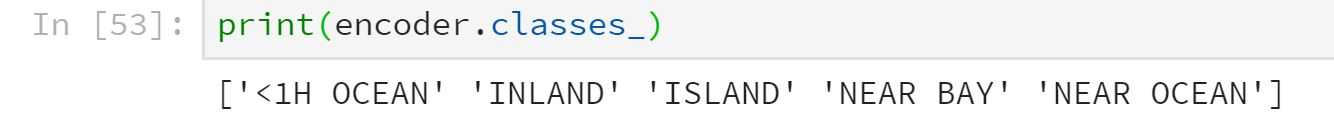
\includegraphics[width = 4in]{encoder_class.JPG}
%\caption{Scatter Matrix}
\end{figure}

这样的处理有一个问题:对上面的例子而言,0和4的距离大于0和1的距离,这个在实际中并没有体现。所以常见的处理方式是,把非数值属性的数值表示由单独向量转化为一个多维数组,用不同位置的0和1来表示不同的属性。Scikit-Learn恰好提供了这样的方法。也就是OneHotEncoder.

\begin{lstlisting}
from sklearn.preprocessing import OneHotEncoder
encoder= OneHotEncoder()
housing_cat_1hot = encoder.fit_transform(housing_cat_encoded.reshape(-1,1))
housing_cat_1hot.toarray()
\end{lstlisting}


\begin{figure}[H]
\centering
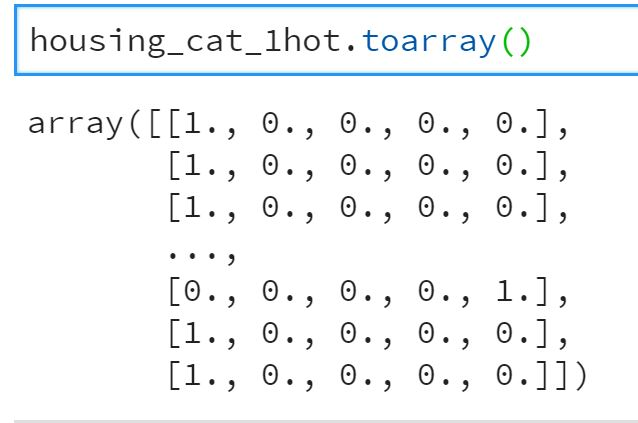
\includegraphics[width = 2in]{Onehot.JPG}
%\caption{Median income versus median house value}
\end{figure}

We can apply both transformations(text to integer,integer to one\underline{ }hot vectors) using the LabelBinarizer class

\begin{lstlisting}
from sklearn.preprocessing import LabelBinarizer
encoder = LabelBinarizer()
housing_cat_1hot = encoder.fit_transform(housing_cat)
housing_cat_1hot
\end{lstlisting}
LabelBinarier method are recommended.

\subsection{Feature Scaling}

Machine Learning algorithms do not perform well when the input numerical attributes have very different scales.The total number of rooms ranges from 6 to 39320 while the median income ranges from 0 to 15.

There are two common ways to get all attribute to have the same scale:min-max scaling and strandardization.
Min-max scaling(很多人叫normaliza):把数据根据最大最小值限定在0到1的范围内。Scikit—learn中的MinMaxScalar就是用来实现这个功能的。

\begin{equation}
x_{new} = \frac{x-x_{min}}{x_{max}-x_{min}}
\end{equation}

Standardization:First,it substracts the mean value and divide by unit variance.Standardization does not bound values to a specific range,which may be problems in some algorithms(neural networks).However standardization is much less affected by outliers.简单说就是,当一组数据中大部分数在1-100之间,当有一个离群点1000时,大量的数据都在一个很小的范围内。Scikit-learn provides a transform called StandardScaler for standardization.

\begin{equation}
x_{new}  = \frac{x-\mu}{\sigma}
\end{equation}

\subsection{Custom Transformers}

通常我们把添加属性的过程写成一个类,而不是大段大段的写成凑得。里面设计好具体的方法,于是就有了下面的代码
\begin{lstlisting}
from sklearn.base import BaseEstimator,TransformerMixin

rooms_ix,bedrooms_ix,population_ix,household_ix = 3,4,5,6

class CombinedAttributesAdder(BaseEstimator,TransformerMixin):
    def __init__(self,add_bedrooms_per_room = True):
        self.add_bedrooms_per_room = add_bedrooms_per_room
    def fit(self,X,y = None):
        return self
    def transform(self,X,y=None):
        rooms_per_household = X[:,rooms_ix]/X[:,household_ix]
        population_per_household = X[:,population_ix]/X[:,household_ix]
        if self.add_bedrooms_per_room:
            bedrooms_per_room = X[:,bedrooms_ix]
            return np.c_[X,rooms_per_household,population_per_household,bedrooms_per_room]
        else:
            return np.c_[X,rooms_per_household,population_per_household]

attr_adder = CombinedAttributesAdder(add_bedrooms_per_room = False)
housing_extra_attribs = adder.transform(housing.values)
\end{lstlisting}

\subsection{Transform pipelines}

Scikit-learn provides the \emph{Pipeline} class to help with such sequences of transformations.Here is a small pipeline for numeerical attribute:
\begin{lstlisting}
from sklearn.pipeline import Pipeline
from sklearn.preprocessing import StandardScaler

num_pipeline = Pipeline([('imputer',Imputer(strategy = "median")),('attribs_adder',CombinedAttributesAdder()),('std_scaler',StandardScaler()),])

housing_num_tr = num_pipeline.fit_transform(housing_num)
\end{lstlisting}

The Pipeline constructor takes a list of name/estimator pairs defining a sequence of steps.顾名思义就是按顺序transform输入,一个的输出作为另一个的输入,按顺序执行。We now have a pipeline for numercial values,we also need to apply the LabelBinarizer on the categorical values.在这里要使用的是FeatureUnion().这里有一点改动,就是用CategoricalEncoder代替LabelBinarier.

\begin{lstlisting}
# Definition of the CategoricalEncoder class, copied from PR #9151.
# Just run this cell, or copy it to your code, do not try to understand it (yet).

from sklearn.base import BaseEstimator, TransformerMixin
from sklearn.utils import check_array
from sklearn.preprocessing import LabelEncoder
from scipy import sparse

class CategoricalEncoder(BaseEstimator, TransformerMixin):
    The input to this transformer should be a matrix of integers or strings,
    denoting the values taken on by categorical (discrete) features.
    The features can be encoded using a one-hot aka one-of-K scheme
    (``encoding='onehot'``, the default) or converted to ordinal integers
    (``encoding='ordinal'``).
    This encoding is needed for feeding categorical data to many scikit-learn
    estimators, notably linear models and SVMs with the standard kernels.
    Read more in the :ref:`User Guide <preprocessing_categorical_features>`.
    Parameters
    ----------
    encoding : str, 'onehot', 'onehot-dense' or 'ordinal'
        The type of encoding to use (default is 'onehot'):
        - 'onehot': encode the features using a one-hot aka one-of-K scheme
          (or also called 'dummy' encoding). This creates a binary column for
          each category and returns a sparse matrix.
        - 'onehot-dense': the same as 'onehot' but returns a dense array
          instead of a sparse matrix.
        - 'ordinal': encode the features as ordinal integers. This results in
          a single column of integers (0 to n_categories - 1) per feature.
    categories : 'auto' or a list of lists/arrays of values.
        Categories (unique values) per feature:
        - 'auto' : Determine categories automatically from the training data.
        - list : ``categories[i]`` holds the categories expected in the ith
          column. The passed categories are sorted before encoding the data
          (used categories can be found in the ``categories_`` attribute).
    dtype : number type, default np.float64
        Desired dtype of output.
    handle_unknown : 'error' (default) or 'ignore'
        Whether to raise an error or ignore if a unknown categorical feature is
        present during transform (default is to raise). When this is parameter
        is set to 'ignore' and an unknown category is encountered during
        transform, the resulting one-hot encoded columns for this feature
        will be all zeros.
        Ignoring unknown categories is not supported for
        ``encoding='ordinal'``.
    Attributes
    ----------
    categories_ : list of arrays
        The categories of each feature determined during fitting. When
        categories were specified manually, this holds the sorted categories
        (in order corresponding with output of `transform`).
    Examples
    --------
    Given a dataset with three features and two samples, we let the encoder
    find the maximum value per feature and transform the data to a binary
    one-hot encoding.
    >>> from sklearn.preprocessing import CategoricalEncoder
    >>> enc = CategoricalEncoder(handle_unknown='ignore')
    >>> enc.fit([[0, 0, 3], [1, 1, 0], [0, 2, 1], [1, 0, 2]])
    ... # doctest: +ELLIPSIS
    CategoricalEncoder(categories='auto', dtype=<... 'numpy.float64'>,
              encoding='onehot', handle_unknown='ignore')
    >>> enc.transform([[0, 1, 1], [1, 0, 4]]).toarray()
    array([[ 1.,  0.,  0.,  1.,  0.,  0.,  1.,  0.,  0.],
           [ 0.,  1.,  1.,  0.,  0.,  0.,  0.,  0.,  0.]])
    See also
    --------
    sklearn.preprocessing.OneHotEncoder : performs a one-hot encoding of
      integer ordinal features. The ``OneHotEncoder assumes`` that input
      features take on values in the range ``[0, max(feature)]`` instead of
      using the unique values.
    sklearn.feature_extraction.DictVectorizer : performs a one-hot encoding of
      dictionary items (also handles string-valued features).
    sklearn.feature_extraction.FeatureHasher : performs an approximate one-hot
      encoding of dictionary items or strings.
    """

    def __init__(self, encoding='onehot', categories='auto', dtype=np.float64,
                 handle_unknown='error'):
        self.encoding = encoding
        self.categories = categories
        self.dtype = dtype
        self.handle_unknown = handle_unknown

    def fit(self, X, y=None):
        """Fit the CategoricalEncoder to X.
        Parameters
        ----------
        X : array-like, shape [n_samples, n_feature]
            The data to determine the categories of each feature.
        Returns
        -------
        self
        """

        if self.encoding not in ['onehot', 'onehot-dense', 'ordinal']:
            template = ("encoding should be either 'onehot', 'onehot-dense' "
                        "or 'ordinal', got %s")
            raise ValueError(template % self.handle_unknown)

        if self.handle_unknown not in ['error', 'ignore']:
            template = ("handle_unknown should be either 'error' or "
                        "'ignore', got %s")
            raise ValueError(template % self.handle_unknown)

        if self.encoding == 'ordinal' and self.handle_unknown == 'ignore':
            raise ValueError("handle_unknown='ignore' is not supported for"
                             " encoding='ordinal'")

        X = check_array(X, dtype=np.object, accept_sparse='csc', copy=True)
        n_samples, n_features = X.shape

        self._label_encoders_ = [LabelEncoder() for _ in range(n_features)]

        for i in range(n_features):
            le = self._label_encoders_[i]
            Xi = X[:, i]
            if self.categories == 'auto':
                le.fit(Xi)
            else:
                valid_mask = np.in1d(Xi, self.categories[i])
                if not np.all(valid_mask):
                    if self.handle_unknown == 'error':
                        diff = np.unique(Xi[~valid_mask])
                        msg = ("Found unknown categories {0} in column {1}"
                               " during fit".format(diff, i))
                        raise ValueError(msg)
                le.classes_ = np.array(np.sort(self.categories[i]))

        self.categories_ = [le.classes_ for le in self._label_encoders_]

        return self

    def transform(self, X):
        """Transform X using one-hot encoding.
        Parameters
        ----------
        X : array-like, shape [n_samples, n_features]
            The data to encode.
        Returns
        -------
        X_out : sparse matrix or a 2-d array
            Transformed input.
        """
        X = check_array(X, accept_sparse='csc', dtype=np.object, copy=True)
        n_samples, n_features = X.shape
        X_int = np.zeros_like(X, dtype=np.int)
        X_mask = np.ones_like(X, dtype=np.bool)

        for i in range(n_features):
            valid_mask = np.in1d(X[:, i], self.categories_[i])

            if not np.all(valid_mask):
                if self.handle_unknown == 'error':
                    diff = np.unique(X[~valid_mask, i])
                    msg = ("Found unknown categories {0} in column {1}"
                           " during transform".format(diff, i))
                    raise ValueError(msg)
                else:
                    # Set the problematic rows to an acceptable value and
                    # continue `The rows are marked `X_mask` and will be
                    # removed later.
                    X_mask[:, i] = valid_mask
                    X[:, i][~valid_mask] = self.categories_[i][0]
            X_int[:, i] = self._label_encoders_[i].transform(X[:, i])

        if self.encoding == 'ordinal':
            return X_int.astype(self.dtype, copy=False)

        mask = X_mask.ravel()
        n_values = [cats.shape[0] for cats in self.categories_]
        n_values = np.array([0] + n_values)
        indices = np.cumsum(n_values)

        column_indices = (X_int + indices[:-1]).ravel()[mask]
        row_indices = np.repeat(np.arange(n_samples, dtype=np.int32),
                                n_features)[mask]
        data = np.ones(n_samples * n_features)[mask]

        out = sparse.csc_matrix((data, (row_indices, column_indices)),
                                shape=(n_samples, indices[-1]),
                                dtype=self.dtype).tocsr()
        if self.encoding == 'onehot-dense':
            return out.toarray()
        else:
            return out
\end{lstlisting}

\begin{lstlisting}
from sklearn.pipeline import FeatureUnion

num_attribs = list(housing_num)
cat_attribs = ["ocean_proximity"]

class DataFrameSelector(BaseEstimator,TransformerMixin):
    def __init__(self,attribute_names):
        self.attribute_names = attribute_names
    def fit(self,X,y=None):
        return self
    def transform(self,X):
        return X[self.attribute_names].values

num_pipeline = Pipeline([('selector',DataFrameSelector(num_attribs)),('imputer',Imputer(strategy="median")),('attr_adder',CombinedAttributesAdder()),('std_scaler',StandardScaler()),])
cat_pipeline = Pipeline([('selector',DataFrameSelector(cat_attribs)),('label_binarizer',CategoricalEncoder(encoding="onehot-dense")),])
full_pipeline = FeatureUnion(transformer_list=[("num_pipeline",num_pipeline),("cat_pipeline",cat_pipeline),])
\end{lstlisting}	

最后这部分代码比较多,其实主要是书上的代码稍稍有点问题,所以就稍稍做了改动,具体可以查看code部分的实现,但是这都不是最重要的,最重要的其实是对pipeline的掌握,其实这里无非就是把之前的step by step的内容改成了pipeline的形式。接下来,我们就要开始最核心部分的学习了,我们花了很长的时间去做准备工作,真正的模型构建及数据处理,由于sklearn封装的原因,显得比较单薄。

\section{Select and Train a Model}

\subsection{Training and Evaluating on the Training Set}

Let's first train a Linear Regression Model.
\begin{lstlisting}
from sklearn.linear_model import LinearRegression

lin_reg = LinearRegression()
lin_reg.fit(housing_prepared,housing_labels)
\end{lstlisting}

It's simple!Let's try it out on a few instance from the training set:

\begin{lstlisting}
some_data = housing.iloc[:5]
some_labels = housing_labels[:5]
some_data_prepared = full_pipeline.transform(some_data)
print(lin_reg.predict(some_data_prepared))
print(list(some_labels))
\end{lstlisting}

It works!Although the prediction are not exactly accurate.Let's evaluate the RMSE(标准差) on the whole training set using Scikit-Learn's mean\underline{ }squared\_error function.

\begin{lstlisting}
from sklearn.metrics import mean_squared_error

housing_predictions = lin_reg.predict(housing_prepared)
lin_mse = mean_squared_error(housing_labels,housing_predictions)
lin_rmse = np.sqrt(lin_mse)
lin_rmse
\end{lstlisting}

The result is 67842.Well,this is better than nothing but clearly not a great score.As we said before,underfitting is the reason why leading to the low accuracy.We can selecting a more powerful model,feeding better feature or reducing the constraints on the model.Let's first try a more complex model to see how it does.

Let's train a DecisionTreeRegressor.This is a more powerful model,capable of finding complex nonlinear relationship in the data.Then,let's evaluate it on the training set:

\begin{lstlisting}
from sklearn.tree import DecisionTreeRegressor

tree_reg = DecisionTreeRegressor()
tree_reg.fit(housing_prepared,housing_labels)
housing_predictions = tree_reg.predict(housing_prepared)
tree_mse  =mean_squared_error(housing_predictions,housing_labels)
tree_rmse = np.sqrt(tree_mse)
tree_rmse
\end{lstlisting}


\begin{figure}[H]
\centering
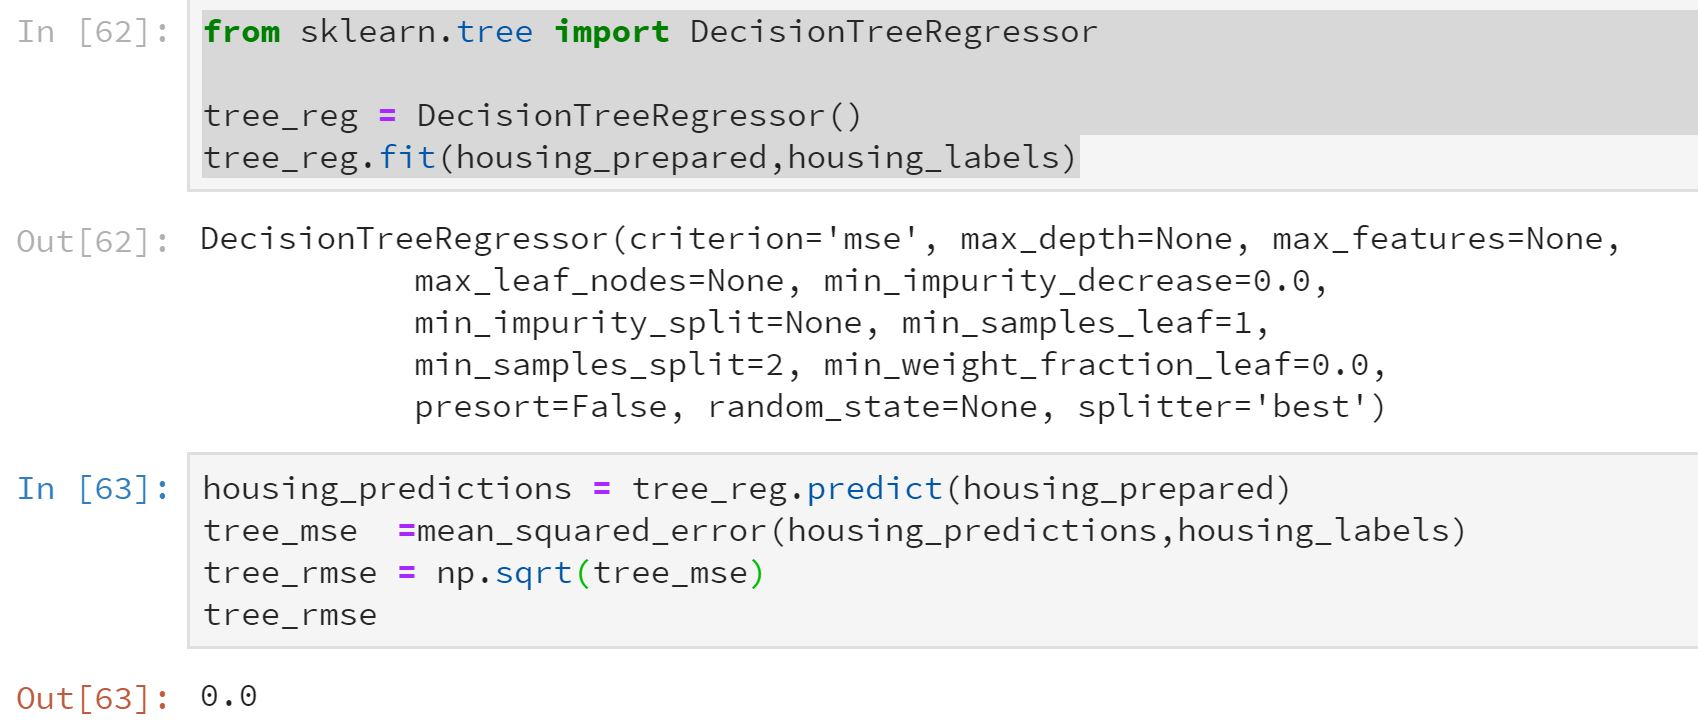
\includegraphics[width = 4in]{treeregressorJPG.JPG}
\caption{bizarre result}
\end{figure}


Of course it is much more likely that the model has badly overfitting problem.

\subsection{Better Evaluation Using Cross-Validation}

One way to evaluate the decision Tree would be to use the train\_test\_split function to split the training set into a smaller training set and a vaildation set,then train your models against the smaller training set and evaluate them against the vaildation set.

A great alternative is to use Scikit-Learn's cross-vaildation feature.The following code performs \emph{K-fold} cross-vaildation:简而言之,就是训练集分成10份,分别用一份来验证,其余9份来训练,一共做十次。输出结果是一个array,把十次的结果输出。

\begin{lstlisting}
from sklearn.model_selection import cross_val_score

scores = cross_val_score(tree_reg,housing_prepared,housing_labels,scoring="neg_mean_squared_error",cv=10)
rmse_scores = np.sqrt(-scores)
\end{lstlisting} 

在这里使用的是均方根误差,也就是把预测值和实际值之间求一个MSE。

\begin{figure}[H]
\centering
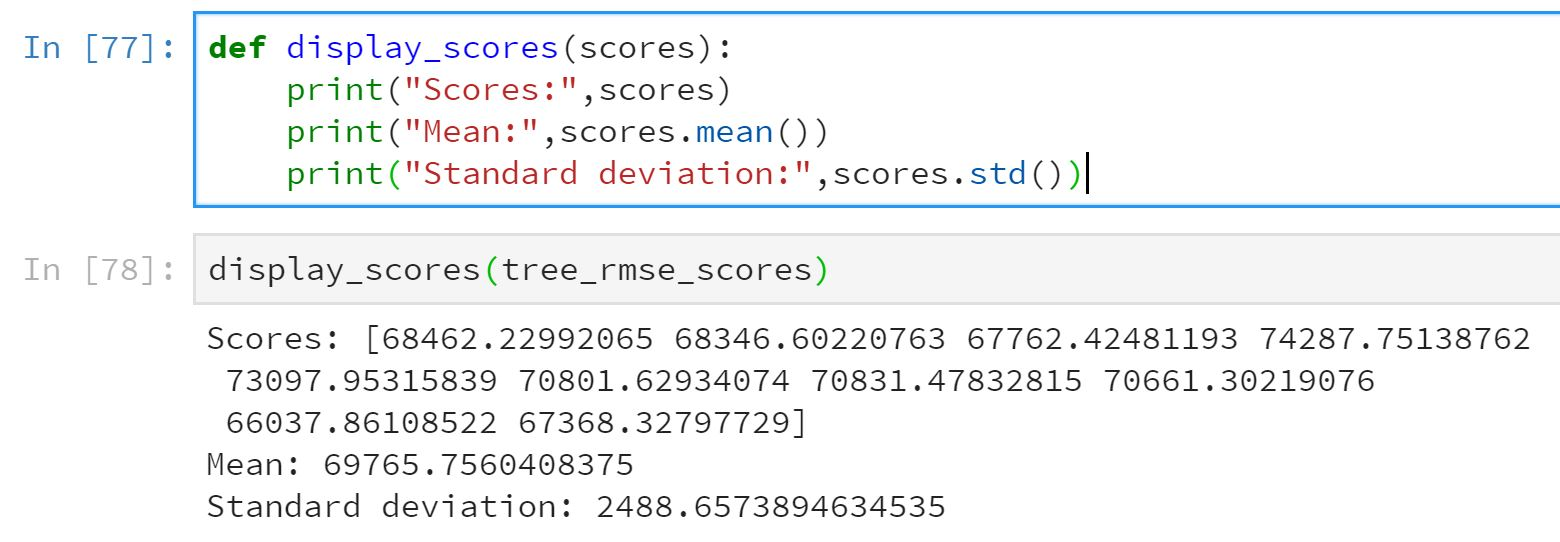
\includegraphics[width = 4in]{cross_val.JPG}
\caption{Cross-Vaildation of DecisionTreeRegressor}
\end{figure}

The decision tree doesn't look good as it did earlier.In fact,it seems to perform worse than the Linear Regression Model.Let's compute the same scores for the Linear Regression model:
\begin{lstlisting}
lin_scores = cross_val_score(lin_reg,housing_prepared,housing_labels,scoring="neg_mean_squared_error",cv=10)
lin_rmse_scores = np.sqrt(-lin_scores)
display_scores(lin_rmse_scores)
\end{lstlisting}

\begin{figure}[H]
\centering
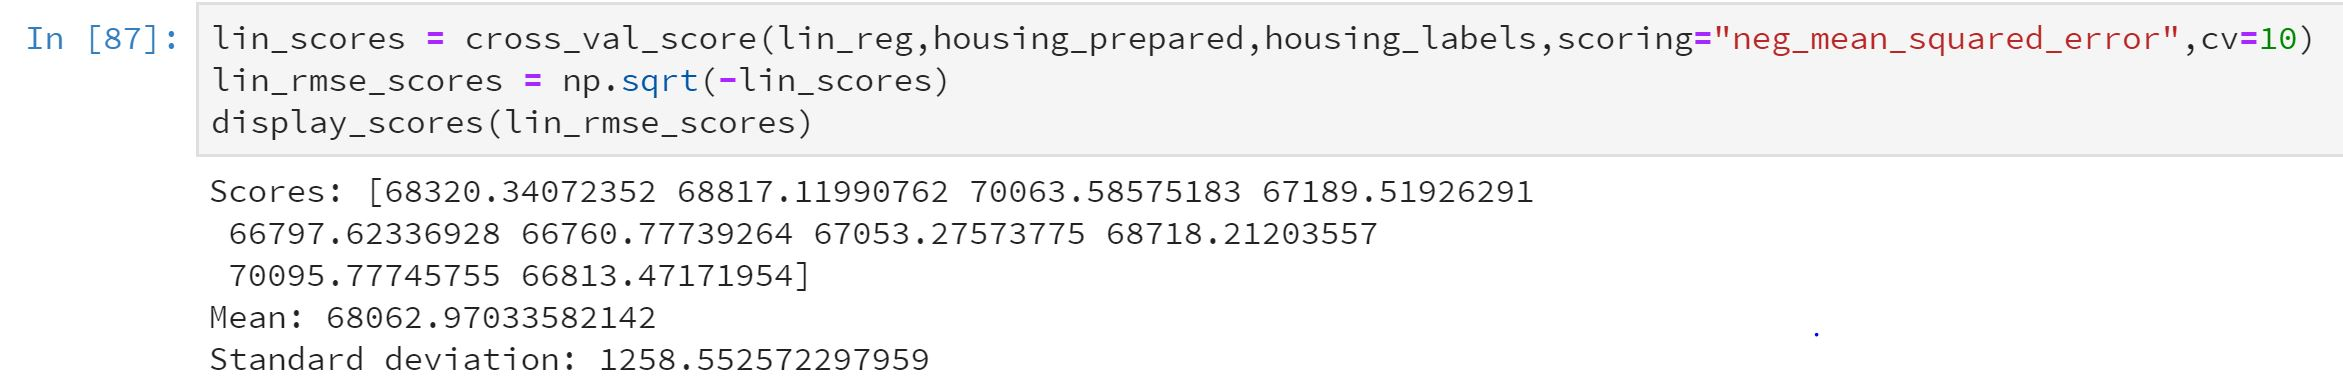
\includegraphics[width = 4in]{lin_cross_val.JPG}
\caption{Cross-Vaildation of Linear Regression}
\end{figure}

可以看出,决策树模型的精度比起线性回归更差。

Let's try one last model:RandomForestRegressor.更多内容,后面章节会细讲。
\begin{lstlisting}
from sklearn.ensemble import RandomForestRegressor
forest_reg = RandomForestRegressor()
forest_reg.fit(housing_prepared,housing_labels)
scores = cross_val_score(forest_reg,housing_prepared,housing_labels,scoring="neg_mean_squared_error",cv=10)
forest_rmse_scores = np.sqrt(-scores)
display_scores(forest_rmse_scores)
\end{lstlisting}

\begin{figure}[H]
\centering
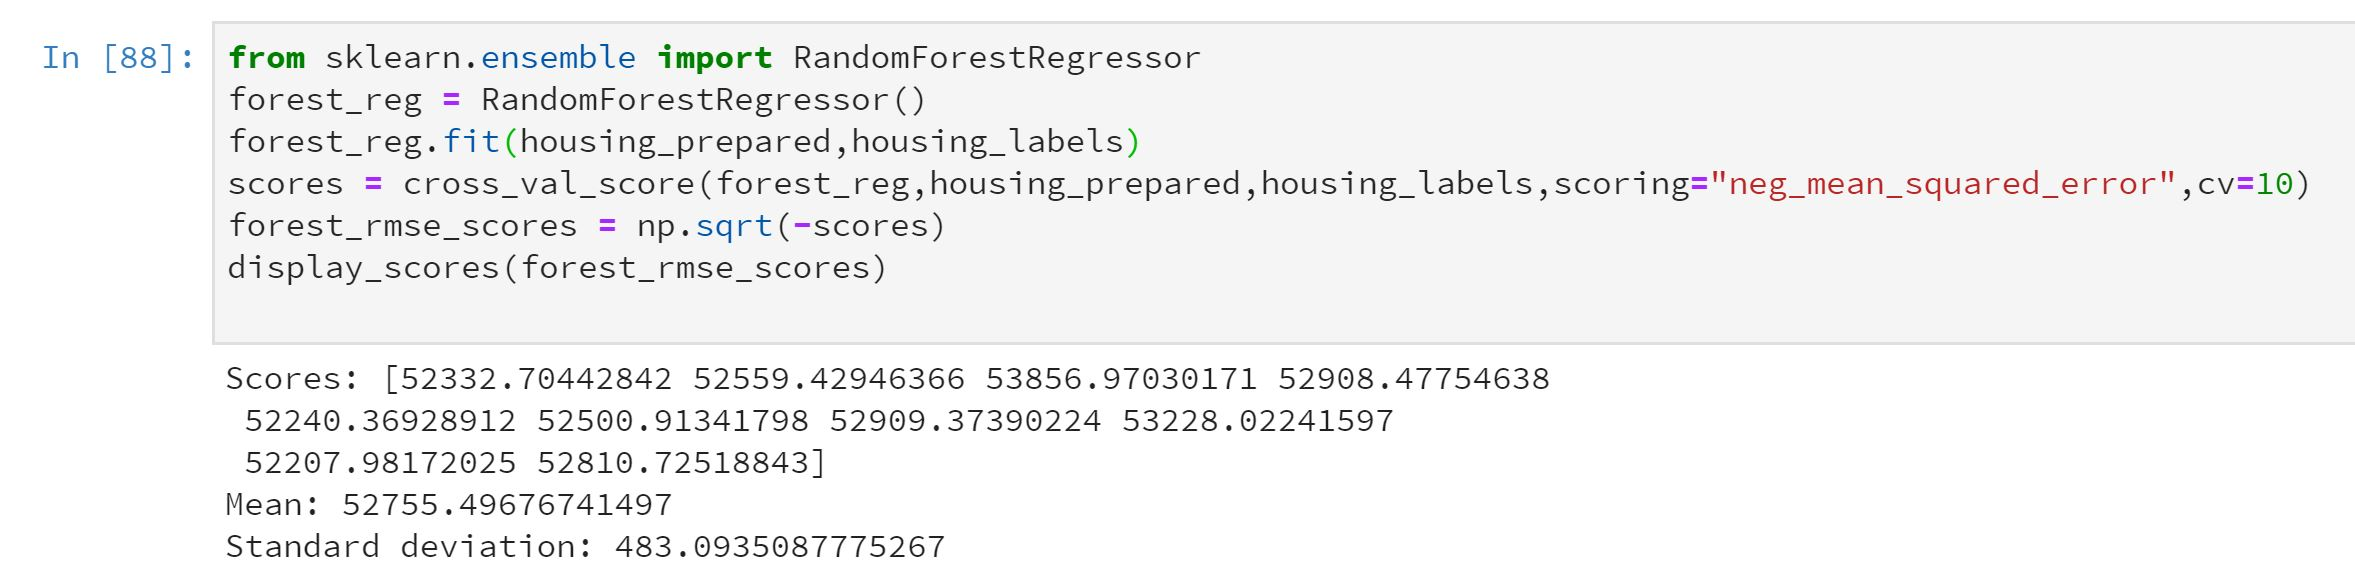
\includegraphics[width = 6in]{forest_val.JPG}
\caption{Cross-Vaildation of RandomForestRegressor}
\end{figure}

通过结果可以看出,预测的结果和实际还是有着较大的差距。因此,这里还是Overfitting了。我们要不就是简化模型,在要不就是获取更多数据。在这里仅仅测试这几个方法,当然可以尝试的方法还有很多。


\section{Fine-Tune Your Model}

Let's assume we have a list of promising models.We need to fine-tune them.

\subsection{Grid Search}

One way to do that is to fiddle with the hyperparameters,until you find the a great combinationof hyperparameter values.We should get Scikit-Learn's GridSearchCV to search for us.

\begin{lstlisting}
from sklearn.model_selection import GridSearchCV

para_grid = [{'n_estimators':[3,10,30],'max_features':[2,4,6,8]},{'bootstrap':[False],'n_estimators':[3,10],'max_features':[2,3,4]}]
forest_reg = RandomForestRegressor()
grid_search = GridSearchCV(forest_reg,para_grid,cv=5,scoring='neg_mean_squared_error')
grid_search.fit(housing_prepared,housing_labels)
\end{lstlisting}

在这里简单说明一下,更详细的将会在后面说到。这里做的就是数据的组合,穷举所有可能的组合。在上面的例子中,首先再第一个字典中衡量$3*4=12$种组合。接下来在第二个字典中穷举$2*3=6$种组合。只是在这里的bootstrap参数被设为False。接下来这18种不同的组合中的每一种都会训练五次(5 times fold cross vaildation).共计90轮训练。

\begin{figure}[H]
\centering
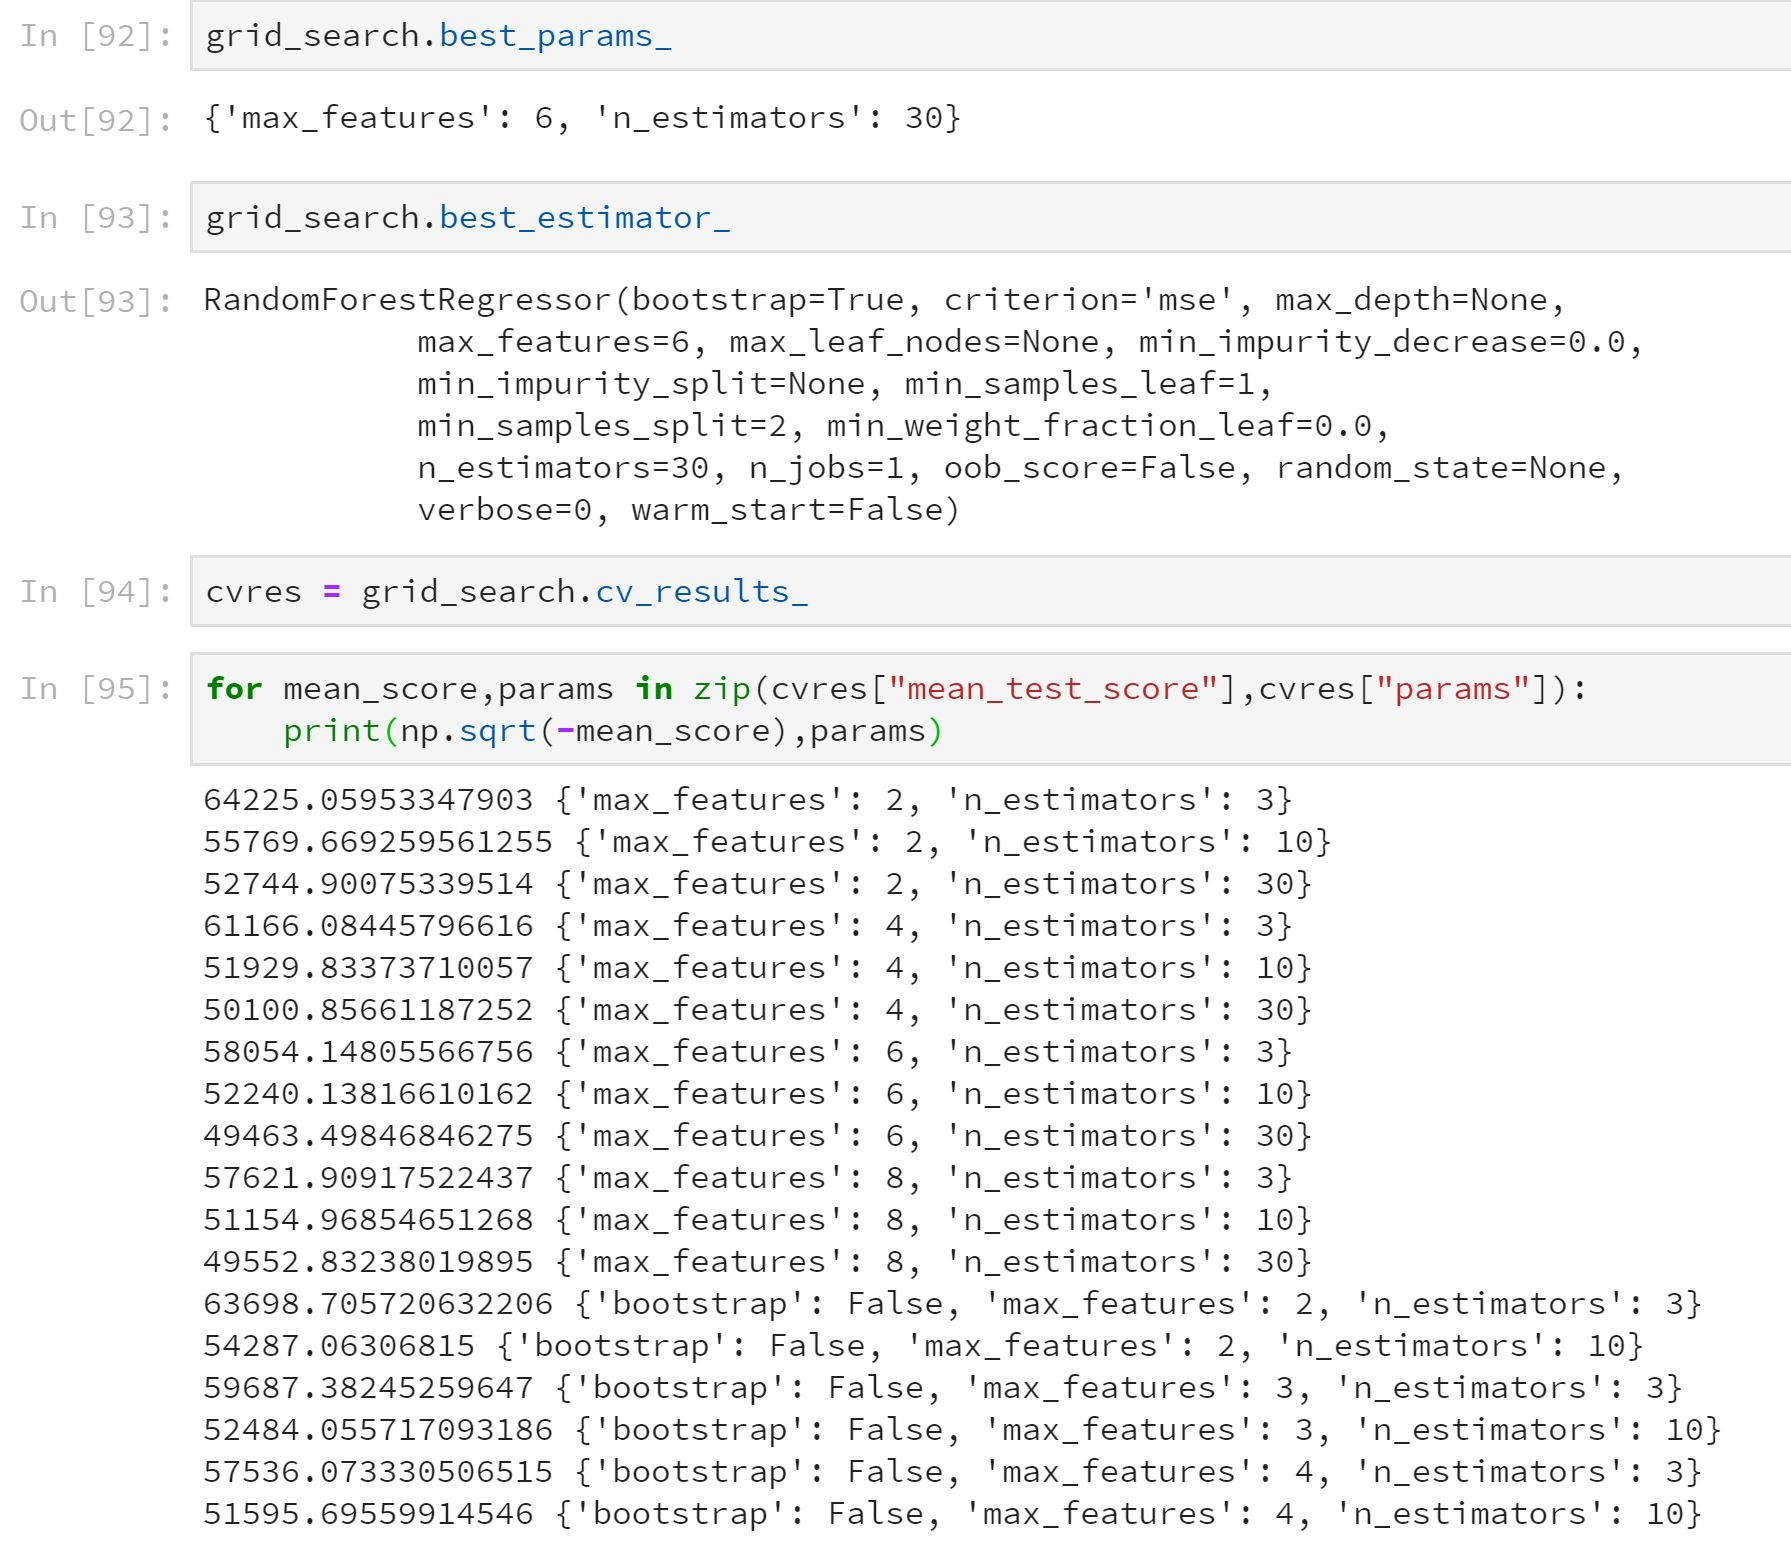
\includegraphics[width = 4.5in]{grid.JPG}
\caption{Grid Search}
\end{figure}

可以看出,最好的情况,RMSE为49959,比之前的结果略好一点(52634)。

\subsection{Randomized Search}
刚才的方法好归好,但是可以想见的是,当attributes过多的时候,这个循环的次数就会非常大,复杂度极高。这时候就会用到RandomizedSearchCV.用法类似,不再赘述。

\subsection{Ensemble Methods}

另一个提高精度的方法就是使用不同模型的组合。这个将在第七章讲。

\subsection{Analyze the Best Models and Their Errors}

通过上面的分析之后,我们看看这些重要的特性是什么


\begin{lstlisting}
feature_importance = grid_search.best_estimator_.feature_importances_
extra_attribs = ["rooms_per_hhold","pop_per_hhold","bedrooms_per_room"]
cat_one_hot_attribs = list(encoder.classes_)
attributes = num_attribs+extra_attribs+cat_one_hot_attribs
sorted(zip(feature_importance,attributes),reverse=True)
\end{lstlisting}

\begin{figure}[H]
\centering
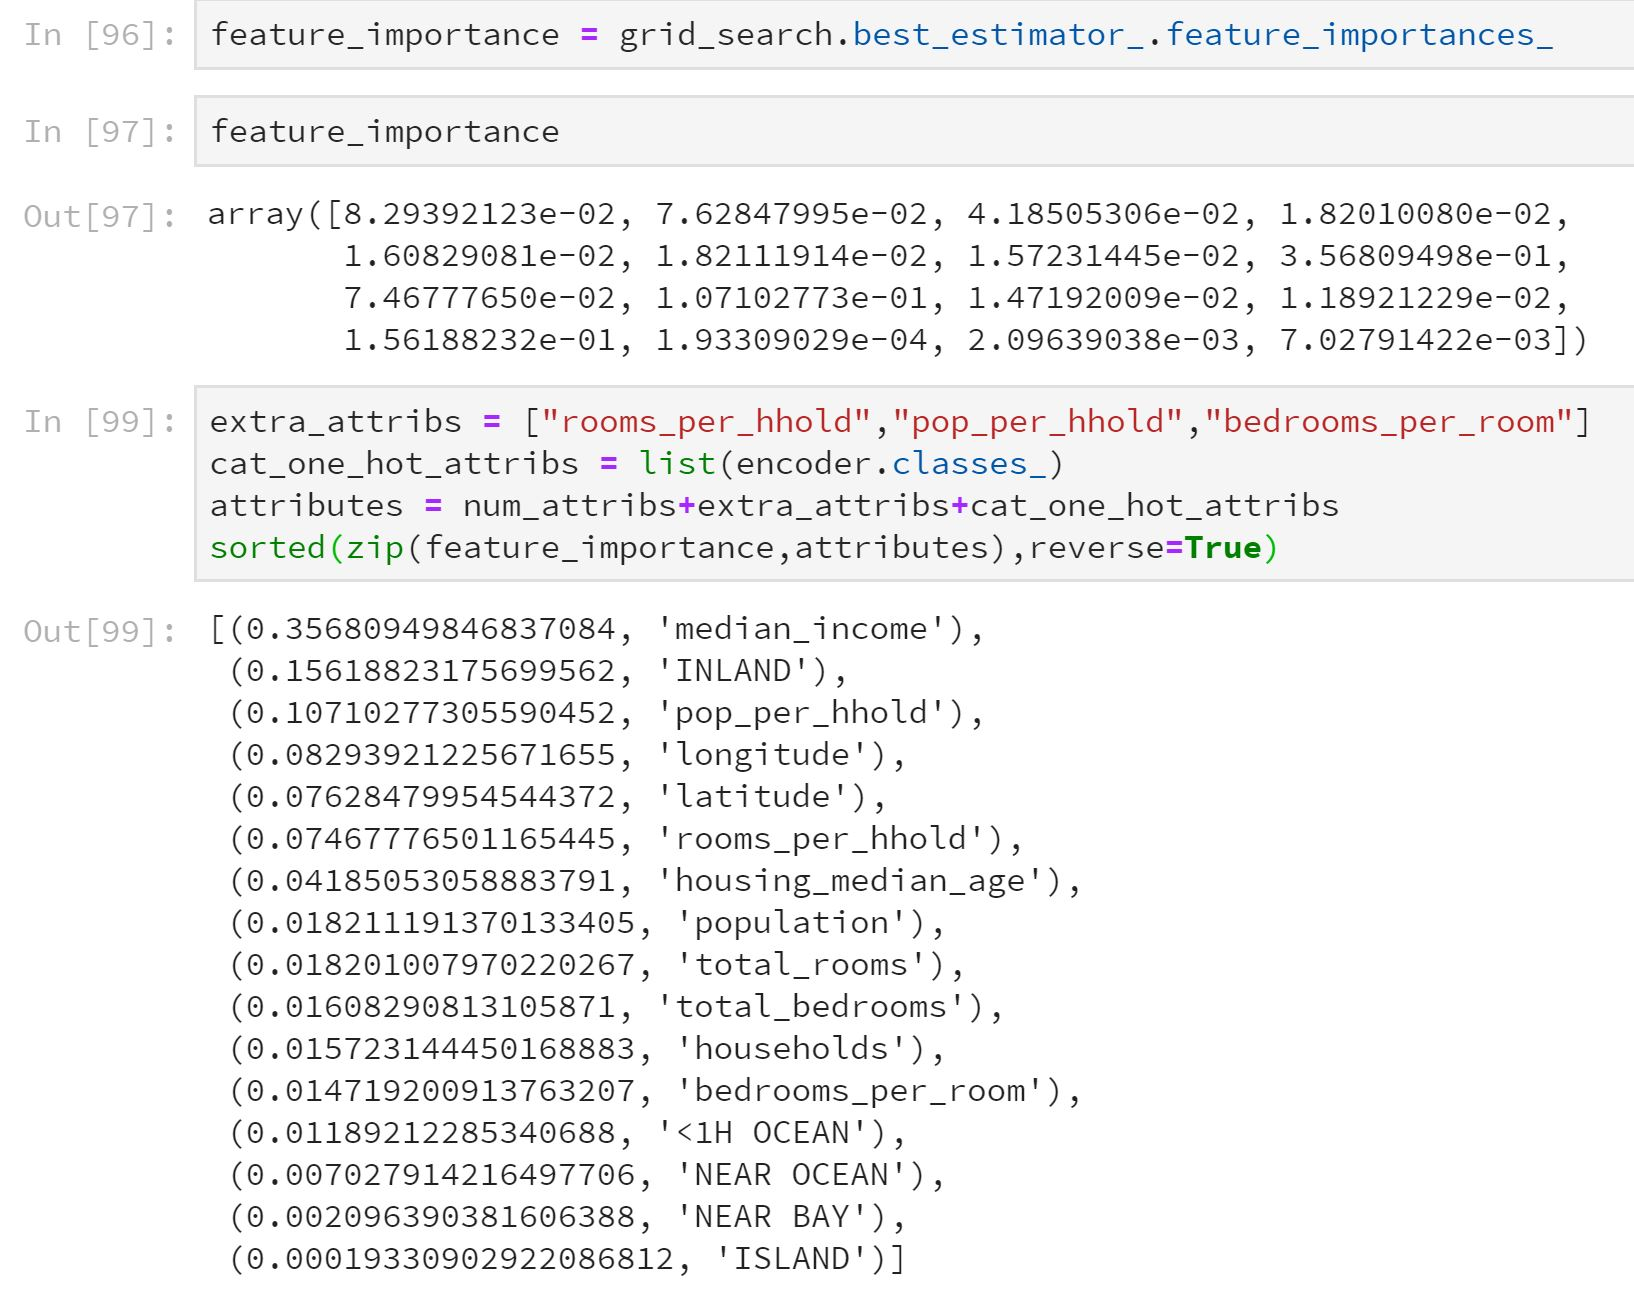
\includegraphics[width = 5in]{feature_imp.JPG}
\caption{Feature importance}
\end{figure}

\subsection{Evaluate Your System on the Test Set}

\begin{lstlisting}
final_model = grid_search.best_estimator_

X_test = strat_test_set.drop("median_house_value",axis = 1)
y_test = strat_test_set["median_house_value"].copy()

X_test_prepared = full_pipeline.transform(X_test)
final_prediction = final_model.predict(X_test_prepared)

final_mse = mean_squared_error(y_test,final_prediction)
final_rmse = np.sqrt(final_mse)
\end{lstlisting}

最后的结果是50014,评估结果通常要比交叉验证的效果差一点,如果你之前做过很多超参数微调(因为你的系统在验证集上微调,得到了不错的性能,通常不会在未知的数据集上有同样好的效果)。这个例子不属于这种情况,但是当发生这种情况时,我们一定要忍住不要调节超参数,使测试集的效果变好;这样的提升不能推广到新数据上。

\section{Launch,Monitor and Maintain Your System}

这部分没有什么特别重要的内容。


\section{Try it Out}

希望这一章能告诉你机器学习项目是什么样的,我们能用学到的工具训练一个好系统。你已经看到,大部分的工作是数据准备步骤、搭建监测工具、建立人为评估的流水线和自动化定期模型训练,当然,最好能了解整个过程、熟悉三或四种算法,而不是在探索高级算法上浪费全部时间,导致在全局上的时间不够。

有机会去kaggle做做东西。第二章就这样结束了。


\end{document}
